\documentclass[pdflatex,iicol,sn-mathphys-num]{sn-jnl}

\usepackage{graphicx}
\usepackage{booktabs}
\usepackage{amsmath,amssymb}
\usepackage{xcolor}
\usepackage{url}

\raggedbottom

\makeatletter
\@ifundefined{pacs}{
  \newcommand{\pacs}[2][]{\par\smallskip\noindent\textbf{#1:} #2\par}
}{}
\makeatother

\begin{document}

\title[Trace-Driven Proactive Autoscaling for Cluster Workloads]{Trace-Driven Proactive Autoscaling for Cluster Workloads via Multi-Horizon Forecasting}

\author*[1]{\fnm{Jinchun} \sur{Liu}}\email{ljc20041122@qq.com}

\affil*[1]{\orgdiv{Hainan International College}, \orgname{Communication University of China}, \orgaddress{\city{Beijing}, \postcode{100024}, \country{China}}}

\abstract{Reactive autoscaling is easy to deploy but often responds too late. This study evaluates a reproducible predictive alternative on public Alibaba traces using aggregate, machine-level, transfer, and broad service-level evidence. The pipeline couples leakage-free multi-horizon forecasting with a trace-driven controller that consumes median and upper-quantile predictions. On the aggregate series, linear regression achieves the lowest average MAE (3.514), while \texttt{UA-MSTCN-Lite} remains competitive and provides calibrated $P90$ coverage of 0.920, 0.867, and 0.868 at the 1-, 5-, and 10-minute horizons. A 12-machine cohort and a 3-fold zero-shot cross-machine benchmark confirm that simple linear structure remains difficult to beat for point prediction. A broad audited service cohort of 139 \texttt{app\_du} groups, extracted from the official container tables and a full mirrored pass over \texttt{container\_usage}, changes the service-level headline: linear regression becomes the strongest average point forecaster (MAE 32.571), while \texttt{UA-MSTCN-Lite} retains useful $P90$ coverage of 0.921, 0.896, and 0.877. Against reactive control, predictive control raises mean SLA violation from 0.017 to 0.031 and scaling actions from 249.0 to 399.4; mean over-provisioning falls from 56.31 to 53.68, but the paired service bootstrap confidence interval crosses zero. Public traces therefore support reproducible predictive-autoscaling evaluation and boundary mapping, but not a claim that the current shared global predictive policy is uniformly better across services.
}

\keywords{cluster computing, workload forecasting, proactive autoscaling, Alibaba trace, resource management}

\pacs[MSC Classification]{68M14, 68M20, 90B15}

\maketitle

\section{Introduction}
Large production clusters increasingly rely on elastic resource control to balance service quality against resource efficiency. In practice, many production stacks still prefer reactive threshold rules because they are operationally simple and easy to explain \citep{lorido2014review,Burns2016BorgKubernetes,Bernstein2014ContainersCloud}. However, reactive autoscaling often expands capacity only after demand has already surged and contracts capacity only after long idle periods. The result is a recurring trade-off between service-level objective violations and persistent over-provisioning.

Predictive autoscaling is a natural response to this limitation, but the literature still shows two recurring weaknesses. First, many papers evaluate forecasting quality and autoscaling quality separately, which makes it difficult to judge how improved prediction changes control trade-offs in practice. Second, many strong cluster-management studies depend on private traces or platform-specific deployments that are hard to reproduce. This reproducibility gap weakens both empirical comparability and operational credibility.

This problem setting is already visible in prior work on host-load prediction \citep{Dinda2000HostLoad}, container autoscaling \citep{Casalicchio2019ContainerAutoscaling}, and uncertainty-aware workload forecasting with Alibaba and Google traces \citep{Rossi2025UncertaintyAwareForecasting}. Taken together, these studies show that forecasting, autoscaling, and distributed resource management are closely linked, but they also show that forecasting quality, control behavior, and validity threats need to be analyzed jointly rather than in isolation.

The present paper therefore asks a narrower question: can public cluster traces support a reproducible predictive capacity-control evaluation that clarifies when decision trade-offs improve relative to reactive rules without requiring private infrastructure? The study instantiates this question on the Alibaba Cluster Trace Program \citep{alibabaclusterdata2026}, using the \texttt{cluster-trace-v2018} release whose official documentation reports about 4000 machines observed over 8 days \citep{alibabav2018trace}. Public analyses of Alibaba traces have already shown rich workload diversity and nontrivial resource-efficiency structure \citep{Jiang2022Characterizing,guo2019limits,luo2021characterizing}, making the dataset suitable for a trace-driven systems study.

The forecasting layer is coupled explicitly to the control layer. Instead of treating prediction as an isolated machine-learning benchmark, the experimental pipeline routes multi-horizon forecasts into an autoscaling simulator with headroom, cooldown, and safety-margin constraints. This separation keeps the control logic interpretable and allows the forecasting backbone to be replaced later without changing the rest of the evaluation route.

The evidence base is also intentionally broader than a single aggregate benchmark. In addition to the aggregate cluster series, the study includes a 12-machine high-coverage cohort, a cross-machine transfer benchmark, and a rule-based broad service-level cohort extracted from official \texttt{container\_meta} and a full mirrored pass over \texttt{container\_usage}. Aggregate and machine-level results show that simple linear baselines remain strong point predictors, whereas \texttt{UA-MSTCN-Lite} contributes calibrated quantiles that are useful for predictive control. The service-level evidence narrows the construct-validity gap further by testing the same forecasting-to-policy route at an application-level autoscaling unit.

The present implementation is intentionally conservative in what it claims. The forecasting backbone is a lightweight uncertainty-aware surrogate rather than the final deep UA-MSTCN architecture, and the service-level cohort is a rule-based broad benchmark rather than a full service census. These limits are kept explicit so that the results are interpreted as verified evidence for the current implementation, not as unsupported claims about a deeper architecture or a complete production deployment. The contribution is therefore evaluative: a reproducible public-trace benchmark and boundary-mapping study rather than a claim that the current controller or surrogate is universally superior.

This paper makes four evaluation-oriented contributions:
\begin{enumerate}
  \item It formulates predictive cluster capacity control as a reproducible public-trace evaluation problem rather than a private platform study.
  \item It establishes a public-trace benchmark pipeline from Alibaba trace acquisition through aggregate-, machine-, and service-level preprocessing, forecasting, and trace-driven policy simulation.
  \item It contributes a multi-granularity evidence surface spanning aggregate forecasting, machine-level benchmarking, cross-machine transfer, and service-level heterogeneity under one consistent protocol.
  \item It reports a boundary-mapping result for the current predictive route: simple linear baselines remain strong for point prediction, uncertainty-aware quantiles remain useful for control, and broader audited service coverage shows that the current shared global predictive policy is not validated as a service-level improvement route.
\end{enumerate}

The remainder of the paper is organized as follows. Section~2 reviews adjacent work on workload characterization, forecasting, autoscaling, and generalization. Section~3 formalizes the forecasting and control problem. Section~4 describes the dataset routes, preprocessing, models, and evaluation protocol. Section~5 reports the forecasting and policy results. Section~6 discusses validity threats, and Section~7 concludes the paper.


\section{Related Work}
\subsection{Representative precedent studies}

Representative prior studies already span host-load prediction \citep{Dinda2000HostLoad}, container autoscaling and metric selection \citep{Casalicchio2019ContainerAutoscaling}, service-granular microservice resource management \citep{ZargarAzad2023MicroserviceFramework,Puebla2024CdaScaler}, uncertainty-aware workload forecasting with transfer learning \citep{Rossi2025UncertaintyAwareForecasting}, and recent predictive autoscaling frameworks for cloud environments \citep{Zanussi2026LoadAwareAutoscaling}. Together these studies connect forecasting quality, autoscaling behavior, and realistic cluster workloads while emphasizing different layers of that space. Table~\ref{tab:related-positioning} summarizes how the present study differs in data source, control linkage, and evidence surface.

\begin{table*}[t]
  \centering
  \caption{Representative prior studies on cluster forecasting and autoscaling.}
  \label{tab:related-positioning}
  \scriptsize
  \begin{tabular}{p{2.8cm}p{1.8cm}p{1.1cm}p{1.3cm}p{4.0cm}}
    \toprule
    Paper & Data & Forecast & Policy link & Relevance to the present study \\
    \midrule
    Dinda and O'Hallaron~\citep{Dinda2000HostLoad} & Cluster host traces & Yes & No & Establishes early forecasting baselines at the cluster-host level. \\
    Casalicchio~\citep{Casalicchio2019ContainerAutoscaling} & Container experiments & Limited & Yes & Shows that metric choice and autoscaling behavior need to be evaluated together. \\
    Rossi et al.~\citep{Rossi2025UncertaintyAwareForecasting} & Google and Alibaba traces & Yes & Service-level analysis & Demonstrates the relevance of uncertainty-aware forecasting and transfer analysis on public traces. \\
    Present study & Alibaba public trace & Yes & Yes & Couples forecasting, transfer, and trace-driven control under one reproducible public-trace pipeline. \\
    \bottomrule
  \end{tabular}
\end{table*}

\subsection{Trace-driven workload characterization}

Public cluster traces are essential because they allow researchers to evaluate scheduling and resource-management ideas under realistic temporal variation. Google cluster traces played this role for earlier large-scale studies \citep{reiss2012google}. Alibaba later released several trace families that exposed co-located datacenter workloads, batch scheduling behavior, microservice metrics, and GPU-cluster behavior \citep{alibabaclusterdata2026}. Follow-up studies characterized co-located workloads in Alibaba cloud datacenters \citep{Jiang2022Characterizing}, examined resource-efficiency bottlenecks \citep{guo2019limits}, and analyzed large-scale microservice dependencies \citep{luo2021characterizing}. Recent cloud-evaluation work has also emphasized reproducible simulation and policy testing against realistic workloads and traces \citep{Canizares2023Simcan2Cloud}. These studies provide strong descriptive or evaluative evidence, but they do not by themselves close the loop between forecasting and operational scaling decisions.

\subsection{Forecasting for cluster and cloud workloads}

Forecasting methods for systems workloads range from classical time-series models to neural sequence models. Empirical cloud-resource prediction has been studied with statistical and machine-learning methods for more than a decade \citep{islam2012empirical,Dinda2000HostLoad,Calheiros2015ARIMAWorkload}. Proactive provisioning studies then moved toward workload classification, multi-step forecasting, and explicit control relevance \citep{Herbst2014ProactiveProvisioning,Baldan2018WorkloadForecasting,Banerjee2021MultiStepPrediction}. Sequence-learning models such as LSTM \citep{hochreiter1997long,Song2017LSTMHostLoad} and more integrated deep-learning approaches \citep{Bi2021IntegratedDeepLearning} later became common choices for multistep forecasting. Probabilistic or quantile-aware forecasting is especially relevant for control problems because capacity decisions should respond not only to central tendency but also to uncertainty \citep{salinas2020deepar,lim2021temporal,Rossi2025UncertaintyAwareForecasting}. The practical challenge is not simply to achieve lower forecast error, but to expose decision-useful uncertainty without making the pipeline too heavy to reproduce.

\subsection{Predictive autoscaling and uncertainty-aware control}

Autoscaling has a long literature in cloud and grid computing, spanning threshold rules, control-theoretic policies, queuing-based methods, and predictive approaches \citep{lorido2014review,Mao2010DeadlineBudgetAutoscaling}. Container-era systems added new operational layers, including orchestration concerns \citep{Bernstein2014ContainersCloud,Burns2016BorgKubernetes}, proactive traffic-aware scaling \citep{Kim2017ProactiveAutoscaling}, and Docker-specific elasticity mechanisms \citep{AlDhuraibi2017ElasticDocker}. More recent service-granular studies examine resource management and cost-aware autoscaling directly at the microservice level \citep{ZargarAzad2023MicroserviceFramework,Puebla2024CdaScaler}, while framework-oriented studies continue to integrate predictive models into end-to-end cloud autoscaling stacks and report operational gains under their target environments \citep{Zanussi2026LoadAwareAutoscaling}. The common appeal of predictive policies is that they can scale before demand surges, but the common risk is that forecast noise can trigger unstable actions. Uncertainty-aware cloud studies therefore remain relevant because they make safety margins explicit \citep{Minarolli2017UncertaintyPrediction,Rossi2025UncertaintyAwareForecasting}. For this reason, a forecasting paper that never evaluates control outcomes, or a control paper that treats forecasts as opaque oracles, leaves an important systems gap unresolved.

\subsection{Transfer learning and generalization}

Recent workload-prediction papers increasingly discuss generalization across workloads and deployment contexts. This includes transfer-learning surveys \citep{Weiss2016TransferLearning}, time-series transfer frameworks \citep{Ye2018TransferForecasting}, and cloud-specific transfer-learning models \citep{Liu2022TRPredictior,Hao2021TransferQoS}. These studies make clear that generalization is already a substantive concern rather than an optional extension. That context matters for how the present study frames cross-machine transfer evidence and remaining limitations.

\subsection{Position of the present study}

The present study is positioned as an end-to-end public-trace evaluation rather than as a new autoscaling framework. Existing public-trace studies are often descriptive, forecasting studies frequently stop before policy evaluation, and predictive autoscaling studies often depend on private data or platform-specific implementations or emphasize positive framework-specific deployment results \citep{Zanussi2026LoadAwareAutoscaling}. The gap addressed here is a reproducible, trace-driven forecasting-to-control benchmark that can be evaluated end to end using public artifacts while making mixed and negative service-level findings explicit rather than hiding them.


\section{Problem Formulation}
Let $e \in \mathcal{E}$ denote the managed entity under study. Depending on the experiment, $e$ may represent the aggregate cluster, an individual machine, or an application-level service identified by Alibaba's \texttt{app\_du}. For every entity, the time index is discretized to one-minute intervals. The observed demand signal is denoted by $x_{e,t} \in \mathbb{R}_{\ge 0}$.

\paragraph{Entity-level forecasting objective.}
Given a context window of length $L$, the forecasting layer receives
\[
\mathbf{x}_{e,t-L+1:t} = \{x_{e,t-L+1}, x_{e,t-L+2}, \dots, x_{e,t}\},
\]
and predicts future demand at horizons $\mathcal{H}=\{1,5,10\}$ minutes. For each $h \in \mathcal{H}$, the model produces at least two quantiles,
\[
\hat{x}^{(0.5)}_{e,t+h}, \qquad \hat{x}^{(0.9)}_{e,t+h},
\]
which correspond to the median and the upper decision quantile. The median supports conservative scale-in, while the upper quantile supports earlier scale-out under uncertainty.

\paragraph{Demand representation.}
The forecasting formulation is shared across all benchmarks, but the physical meaning of $x_{e,t}$ depends on the entity type. For aggregate and machine-level experiments, $x_{e,t}$ is the observed CPU-utilization signal after one-minute aggregation. For service-level experiments, $x_{e,t}$ is a CPU-core demand proxy obtained by aggregating container-level rows that belong to the same \texttt{app\_du} and summing
\[
\text{cpu\_request\_cores} \times \text{cpu\_utilization}.
\]
This keeps the forecasting route consistent while allowing the control layer to operate on service-relevant load units.

\paragraph{Required-capacity mapping.}
The controller acts on a required-capacity signal rather than on the raw forecast. For aggregate and machine-level experiments, the observed demand is first normalized to the policy capacity space and then converted into a minimum required capacity
\[
c^\star_{e,t} = \max\left((1+\rho)\tilde{x}_{e,t},\; c_{\min}\right),
\]
where $\rho$ is the headroom ratio, $\tilde{x}_{e,t}$ is normalized demand, and $c_{\min}$ is the minimum capacity floor.

For service-level experiments, the same logic is expressed in replica-equivalent units. The required replica-equivalent capacity becomes
\[
c^\star_{e,t} = \max\left(\frac{(1+\rho)x_{e,t}}{r_e},\; c_{\min}\right),
\]
where $r_e$ is the median per-container requested CPU cores for service $e$.
This mapping is important because it places reactive, lagged-tracking, and predictive service policies in the same decision space.

\paragraph{Reactive baseline.}
The reactive policy is threshold-based. If the current utilization exceeds an upper threshold, capacity is increased by at most one step. If utilization falls below a lower threshold, capacity is decreased by at most one step. This approximates the structure of common threshold-driven elasticity controllers and serves as the operational baseline.

\paragraph{Lagged target-tracking baseline.}
The second policy baseline is forecast-free but more explicit than threshold control. It drives the next action directly toward the previous-step required capacity:
\[
\begin{aligned}
c_{e,t+1} = \max\Bigl(&c_{\min},\\
&c_{e,t} + \mathrm{clip}(c^\star_{e,t} - c_{e,t}, -\Delta, \Delta)\Bigr).
\end{aligned}
\]
This policy uses the same minimum-capacity floor and maximum single-step change as the predictive controller, but it has no access to future uncertainty and therefore tests whether naive target chasing is already sufficient.

\paragraph{Predictive policy.}
The predictive controller consumes the two quantile forecasts after mapping them into the same required-capacity space as the reactive and lagged baselines. Scale-out decisions use the upper quantile together with an explicit scale-out margin, while scale-in decisions use the median together with a safety margin and a cooldown constraint:
{\small
\[
\begin{aligned}
c_{e,t+1} &= \min(c_{e,t} + \Delta, \hat{c}^{(0.9)}_{e,t+h}),
&& \text{if scale-out},\\
c_{e,t+1} &= \max(c_{e,t} - \Delta,
  (1+\gamma)\hat{c}^{(0.5)}_{e,t+h}),
&& \text{if scale-in},\\
c_{e,t+1} &= c_{e,t},
&& \text{otherwise}.
\end{aligned}
\]
}
where $\Delta$ is the maximum single-step change and $\gamma$ is the scale-in safety margin. Cooldown suppresses oscillatory scale-in without delaying urgent scale-out.

\paragraph{Forecasting backbone.}
The proposed model family is framed as an uncertainty-aware multi-scale temporal forecaster. In the present experiments, that interface is instantiated by \texttt{UA-MSTCN-Lite}, a paper-specific lightweight quantile-forest surrogate that emits $P50$ and $P90$ forecasts without introducing a heavyweight deep-learning dependency stack. \texttt{UA-MSTCN-Lite} is not the full deep UA-MSTCN architecture; it is the reproducible surrogate used to exercise the forecasting-to-control contract in this revision. The surrounding dataset contract, policy simulator, and evaluation protocol are kept stable so that a deeper temporal backbone can replace this surrogate in later work without changing the rest of the study design.

Concretely, \texttt{UA-MSTCN-Lite} uses a 60-minute history window and predicts the 1-, 5-, and 10-minute horizons. Its feature extractor includes lag values at 1, 2, 3, 5, 10, 15, 20, 30, 45, and 60 minutes; multi-scale windows of 3, 5, 10, 20, 30, and 60 minutes; per-window mean, standard deviation, minimum, maximum, median, 0.1 quantile, 0.9 quantile, endpoint difference, last-minus-mean, and slope; and additional short/long moving-average and volatility differences. Each horizon is fitted with a separate \texttt{RandomForestRegressor} using 200 trees, \texttt{min\_samples\_leaf=3}, \texttt{max\_features="sqrt"}, random seed $42+h$, and \texttt{n\_jobs=-1}. Per-tree predictions define the empirical $P50$ and $P90$ outputs. The $P90$ path is widened by the 0.99 quantile of positive training residuals relative to $P50$, while $P50$ and $P90$ are clipped to the training target support, with the upper path allowed up to 1.10 times the training maximum before the calibration floor. Multi-entity transfer experiments use the same implementation with pooled windows from the training entities.

\paragraph{Calibration objective.}
Because the controller consumes quantiles rather than only point forecasts, the evaluation also measures empirical coverage:
\[
\mathrm{cov}^{(q)}_{e,h} = \frac{1}{N}\sum_{i=1}^{N}\mathbb{I}\left(x_{e,t_i+h} \le \hat{x}^{(q)}_{e,t_i+h}\right),
\]
where $q \in \{0.5, 0.9\}$. Ideally, $P50$ and $P90$ coverage should remain close to 0.5 and 0.9, respectively. Interval width $\hat{x}^{(0.9)}_{e,t+h} - \hat{x}^{(0.5)}_{e,t+h}$ is tracked alongside coverage because overly wide intervals may protect SLA at the cost of resource efficiency.

\paragraph{Optimization targets.}
Forecasting quality is evaluated with MAE, RMSE, MAPE, and pinball-oriented quantile diagnostics. Control quality is evaluated with SLA violation rate, over-provisioning, under-provisioning, scaling-action count, and average reserved capacity. This two-layer evaluation is central to the paper because lower forecast error alone does not imply better autoscaling decisions.


\section{Experimental Setup}
\subsection{Dataset and preprocessing}

The experiments use Alibaba \texttt{cluster-trace-v2018}. According to the official trace documentation, the release contains approximately 4000 machines over 8 days and provides machine-level utilization, container-level usage, and batch-workload tables \citep{alibabav2018trace}. The study uses three routes from this release: an aggregate series derived from \texttt{machine\_usage}, a high-coverage machine cohort derived from the same archive, and an expanded service-level cohort built by combining \texttt{container\_meta} with a full local mirror of \texttt{container\_usage.tar.gz}.

The preprocessing script reads machine-usage CSV records directly from the tar archive, retains the required columns, drops invalid rows, aggregates the workload by timestamp, and emits a compact CSV at one-minute granularity. The output contains:
\begin{itemize}
  \item mean cluster CPU utilization,
  \item mean cluster memory utilization, and
  \item the number of active machines.
\end{itemize}
This design keeps the aggregate route simple enough to audit directly, while the later machine and service routes progressively narrow the construct-validity gap. The service route now uses a verified local mirror of the full \texttt{container\_usage.tar.gz} archive rather than a streamed prefix subset, which removes the earlier dependence on low-\texttt{container\_id} extraction heuristics.

\subsection{High-coverage machine cohort}

To move beyond a single aggregate time series, the experimental pipeline also extracts a high-coverage machine cohort from the same Alibaba artifact. The cohort builder first scans the raw \texttt{machine\_usage.tar.gz} archive, selects the 12 machines with the highest row counts, aggregates their samples to one-minute means, and then reindexes every entity onto the common global minute span. Missing minutes are marked explicitly and filled by interpolation only after selection. The retained machines cover between 93.7\% and 94.7\% of the global minute span, with an average imputation ratio of 5.8\%.

This second dataset is not presented as a full service-level benchmark. Its purpose is narrower and more practical: to test whether the forecasting conclusions observed on the aggregate series collapse immediately when the unit of analysis changes from one cluster-wide series to multiple long-lived machine-level series.

\subsection{Container service cohort}

To narrow the remaining construct-validity gap, the pipeline also extracts an expanded service-level cohort from the official Alibaba container tables. The route starts from \texttt{container\_meta.tar.gz}, which exposes container-to-\texttt{app\_du} membership and per-container request sizes. A full pass over the mirrored \texttt{container\_usage.tar.gz} archive then drops rows with blank container identifiers, maps each retained row back to its parent \texttt{app\_du}, and aggregates service demand to one-minute resolution using both mean utilization and a CPU-core proxy computed from the product of requested cores and observed CPU utilization.

The service route now follows a simpler fixed rule. It first applies a metadata prefilter requiring at least 60 containers and at least 650{,}000 seconds of observed span in \texttt{container\_meta}. It then performs a full usage-profile sweep and retains every \texttt{app\_du} group whose matched-container hit ratio is at least 0.90. After service-minute aggregation and reindexing onto the common global span, the final cohort keeps every profiled candidate whose observed-minute coverage remains at least 0.96 and whose matched-container hit ratio remains at least 0.90. Under this rule, the verified broad service cohort contains 139 \texttt{app\_du} groups, 19{,}419 selected containers, and 19{,}269 matched containers over a common 11{,}520-minute span, with an average observed-minute coverage ratio of 97.27\%, a coverage range of 97.23\%--97.30\%, an average matched-container hit ratio of 99.32\%, and an average imputation ratio of 2.73\%. A dedicated top-10 overlap audit retains all 10 services from the earlier targeted cohort. This is therefore a much broader official-data extension, although it still should not be read as a full population census because the metadata prefilter intentionally excludes smaller and shorter-lived services.

\begin{table}[htbp]
  \centering
  \caption{Summary statistics of the broad Alibaba service-level cohort extracted from the official container tables.}
  \label{tab:service-cohort-stats}
  \small
  \begin{tabular}{lc}
    \toprule
    Item & Value \\
    \midrule
    Services (\texttt{app\_du}) & 139 \\
    Selected containers & 19{,}419 \\
    Matched containers in usage stream & 19{,}269 \\
    Common minute span & 11{,}520 \\
    Mean observed-minute coverage & 0.973 \\
    Coverage range & 0.972--0.973 \\
    Mean container hit ratio & 0.993 \\
    Mean imputation ratio & 0.027 \\
    \bottomrule
  \end{tabular}
\end{table}

\begin{table}[htbp]
  \centering
  \caption{Statistics of the processed aggregate Alibaba \texttt{v2018} workload series.}
  \label{tab:dataset-stats}
  \begin{tabular}{lc}
    \toprule
    Item & Value \\
    \midrule
    Observed one-minute samples & 11{,}208 \\
    Minute-index span & 0--11{,}519 \\
    Mean CPU utilization & 37.996\% \\
    Peak CPU utilization & 78.788\% \\
    Mean memory utilization & 88.007\% \\
    Median active machine count & 3994.917 \\
    \bottomrule
  \end{tabular}
\end{table}

\begin{figure}[htbp]
  \centering
  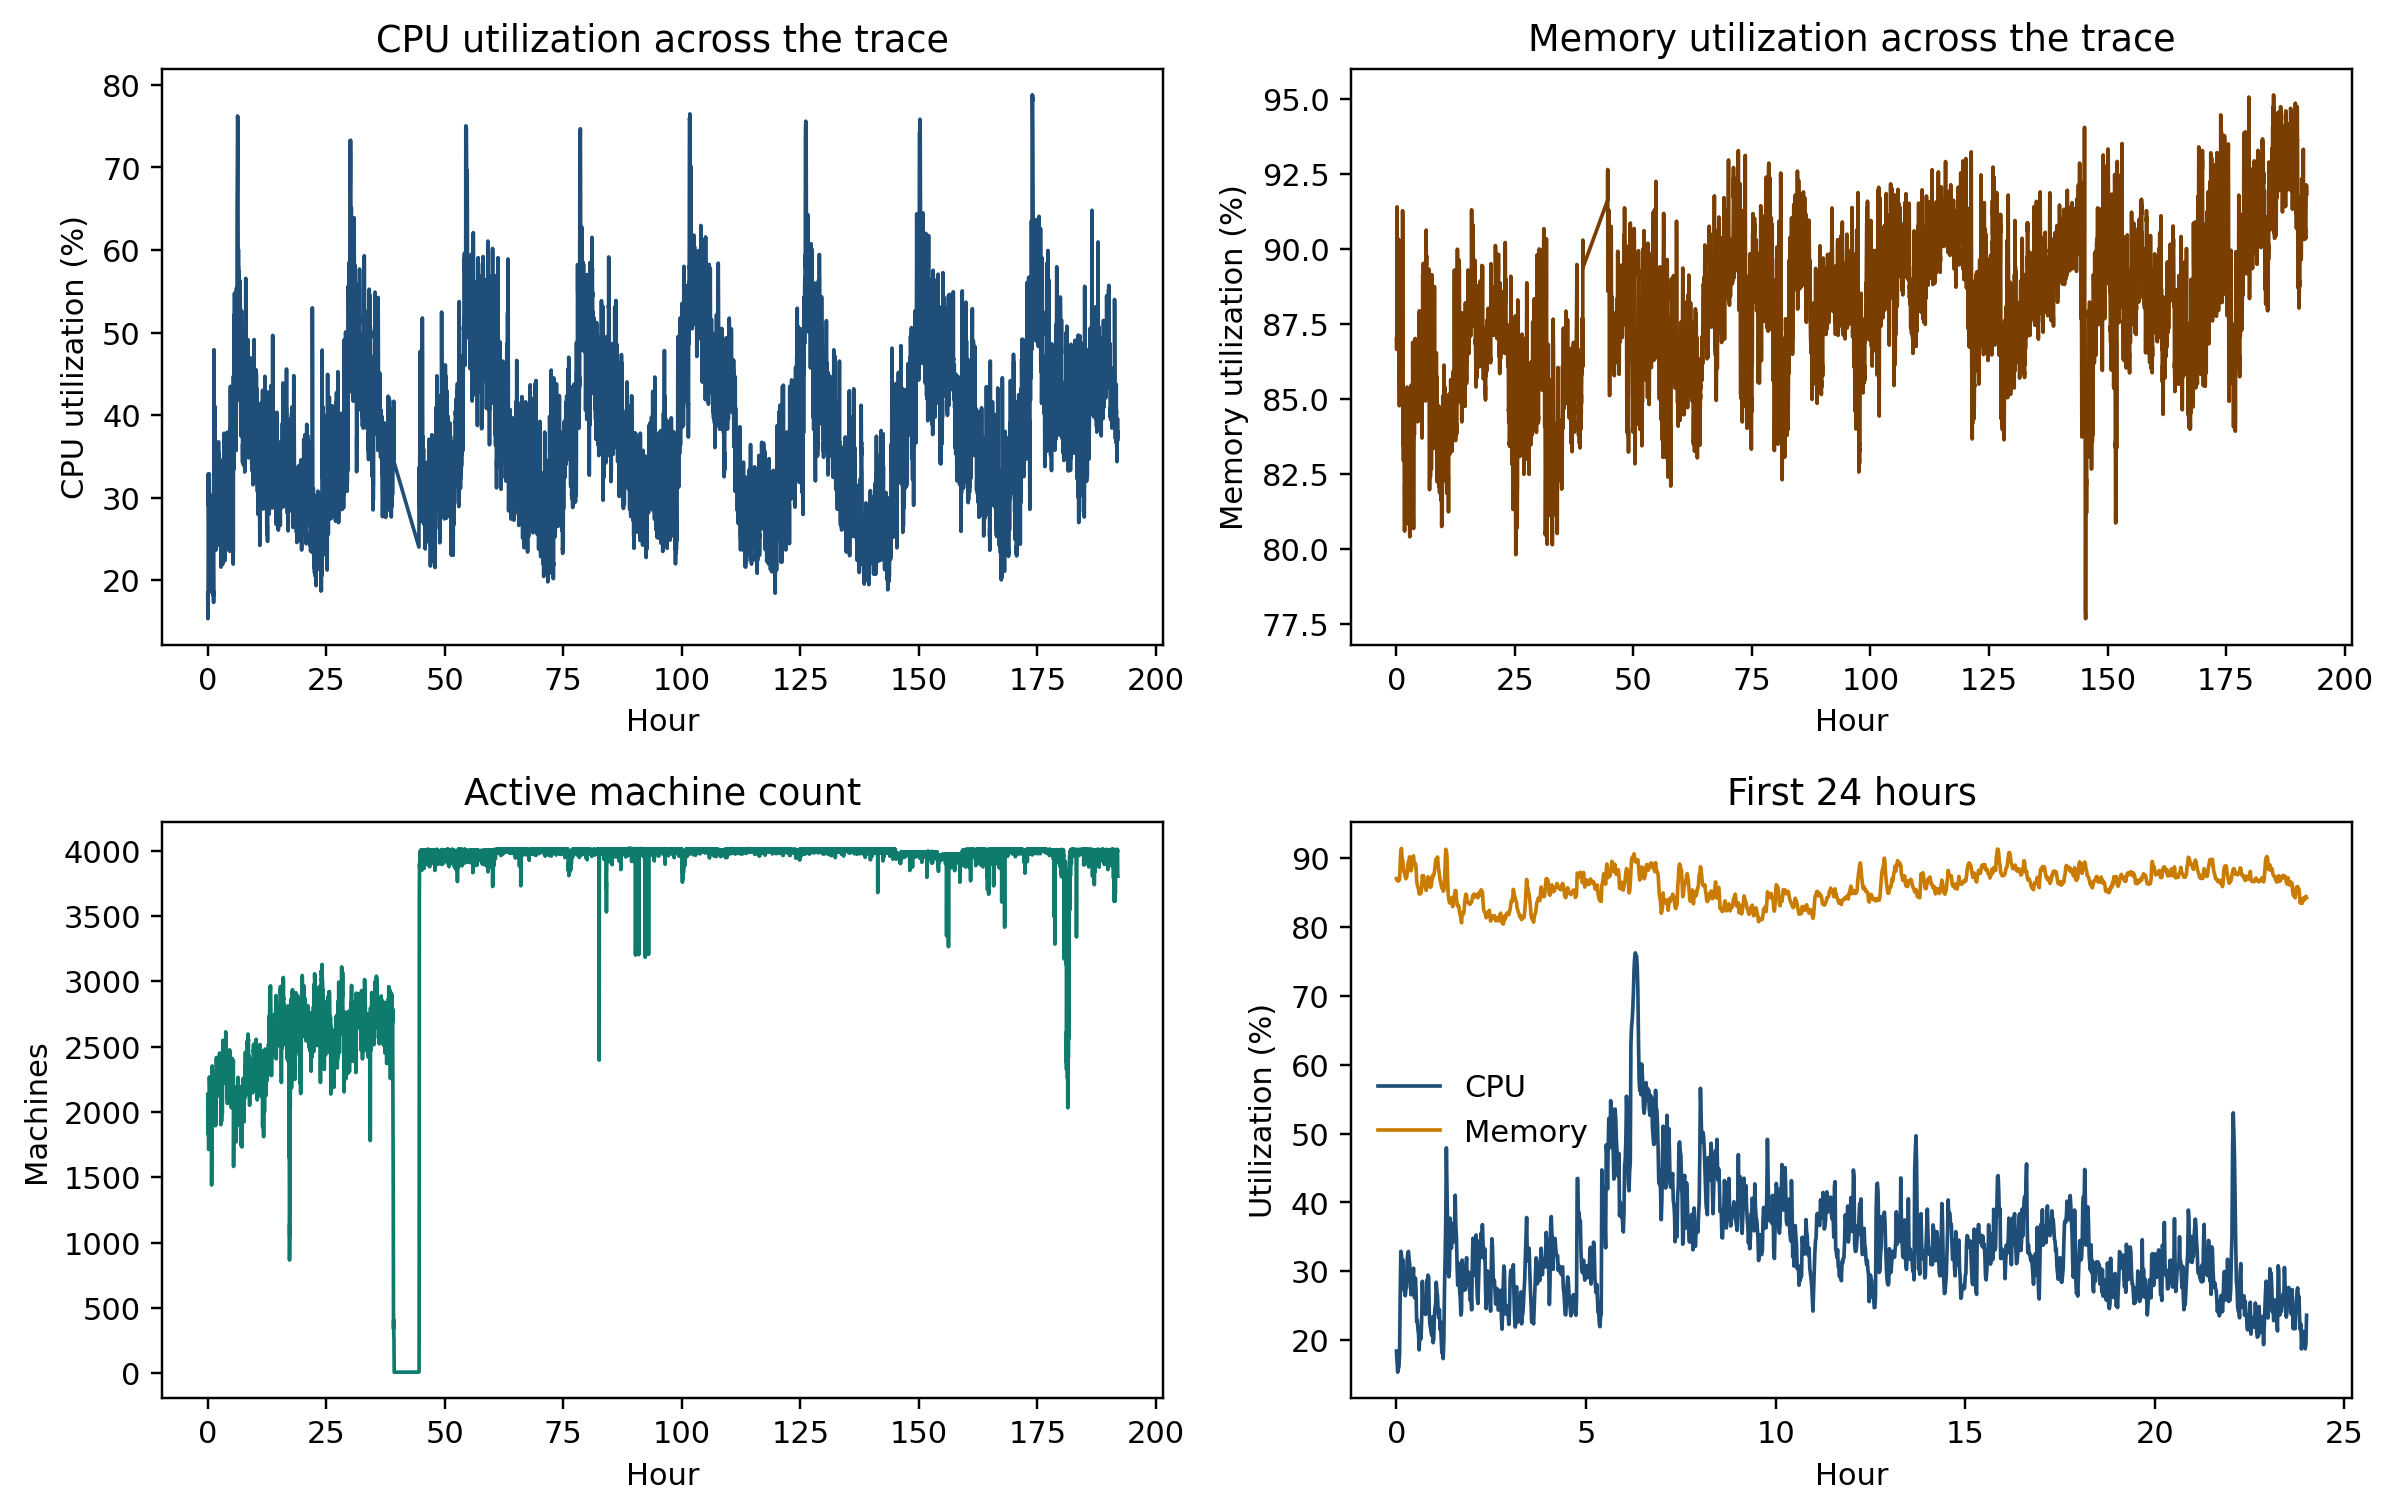
\includegraphics[width=\linewidth]{../experiments/results/figures/cluster_workload_overview.png}
  \caption{Aggregate workload overview across the processed Alibaba \texttt{v2018} series, including CPU, memory, active-machine counts, and the first-day zoom.}
  \label{fig:workload-overview}
\end{figure}

\begin{figure}[htbp]
  \centering
  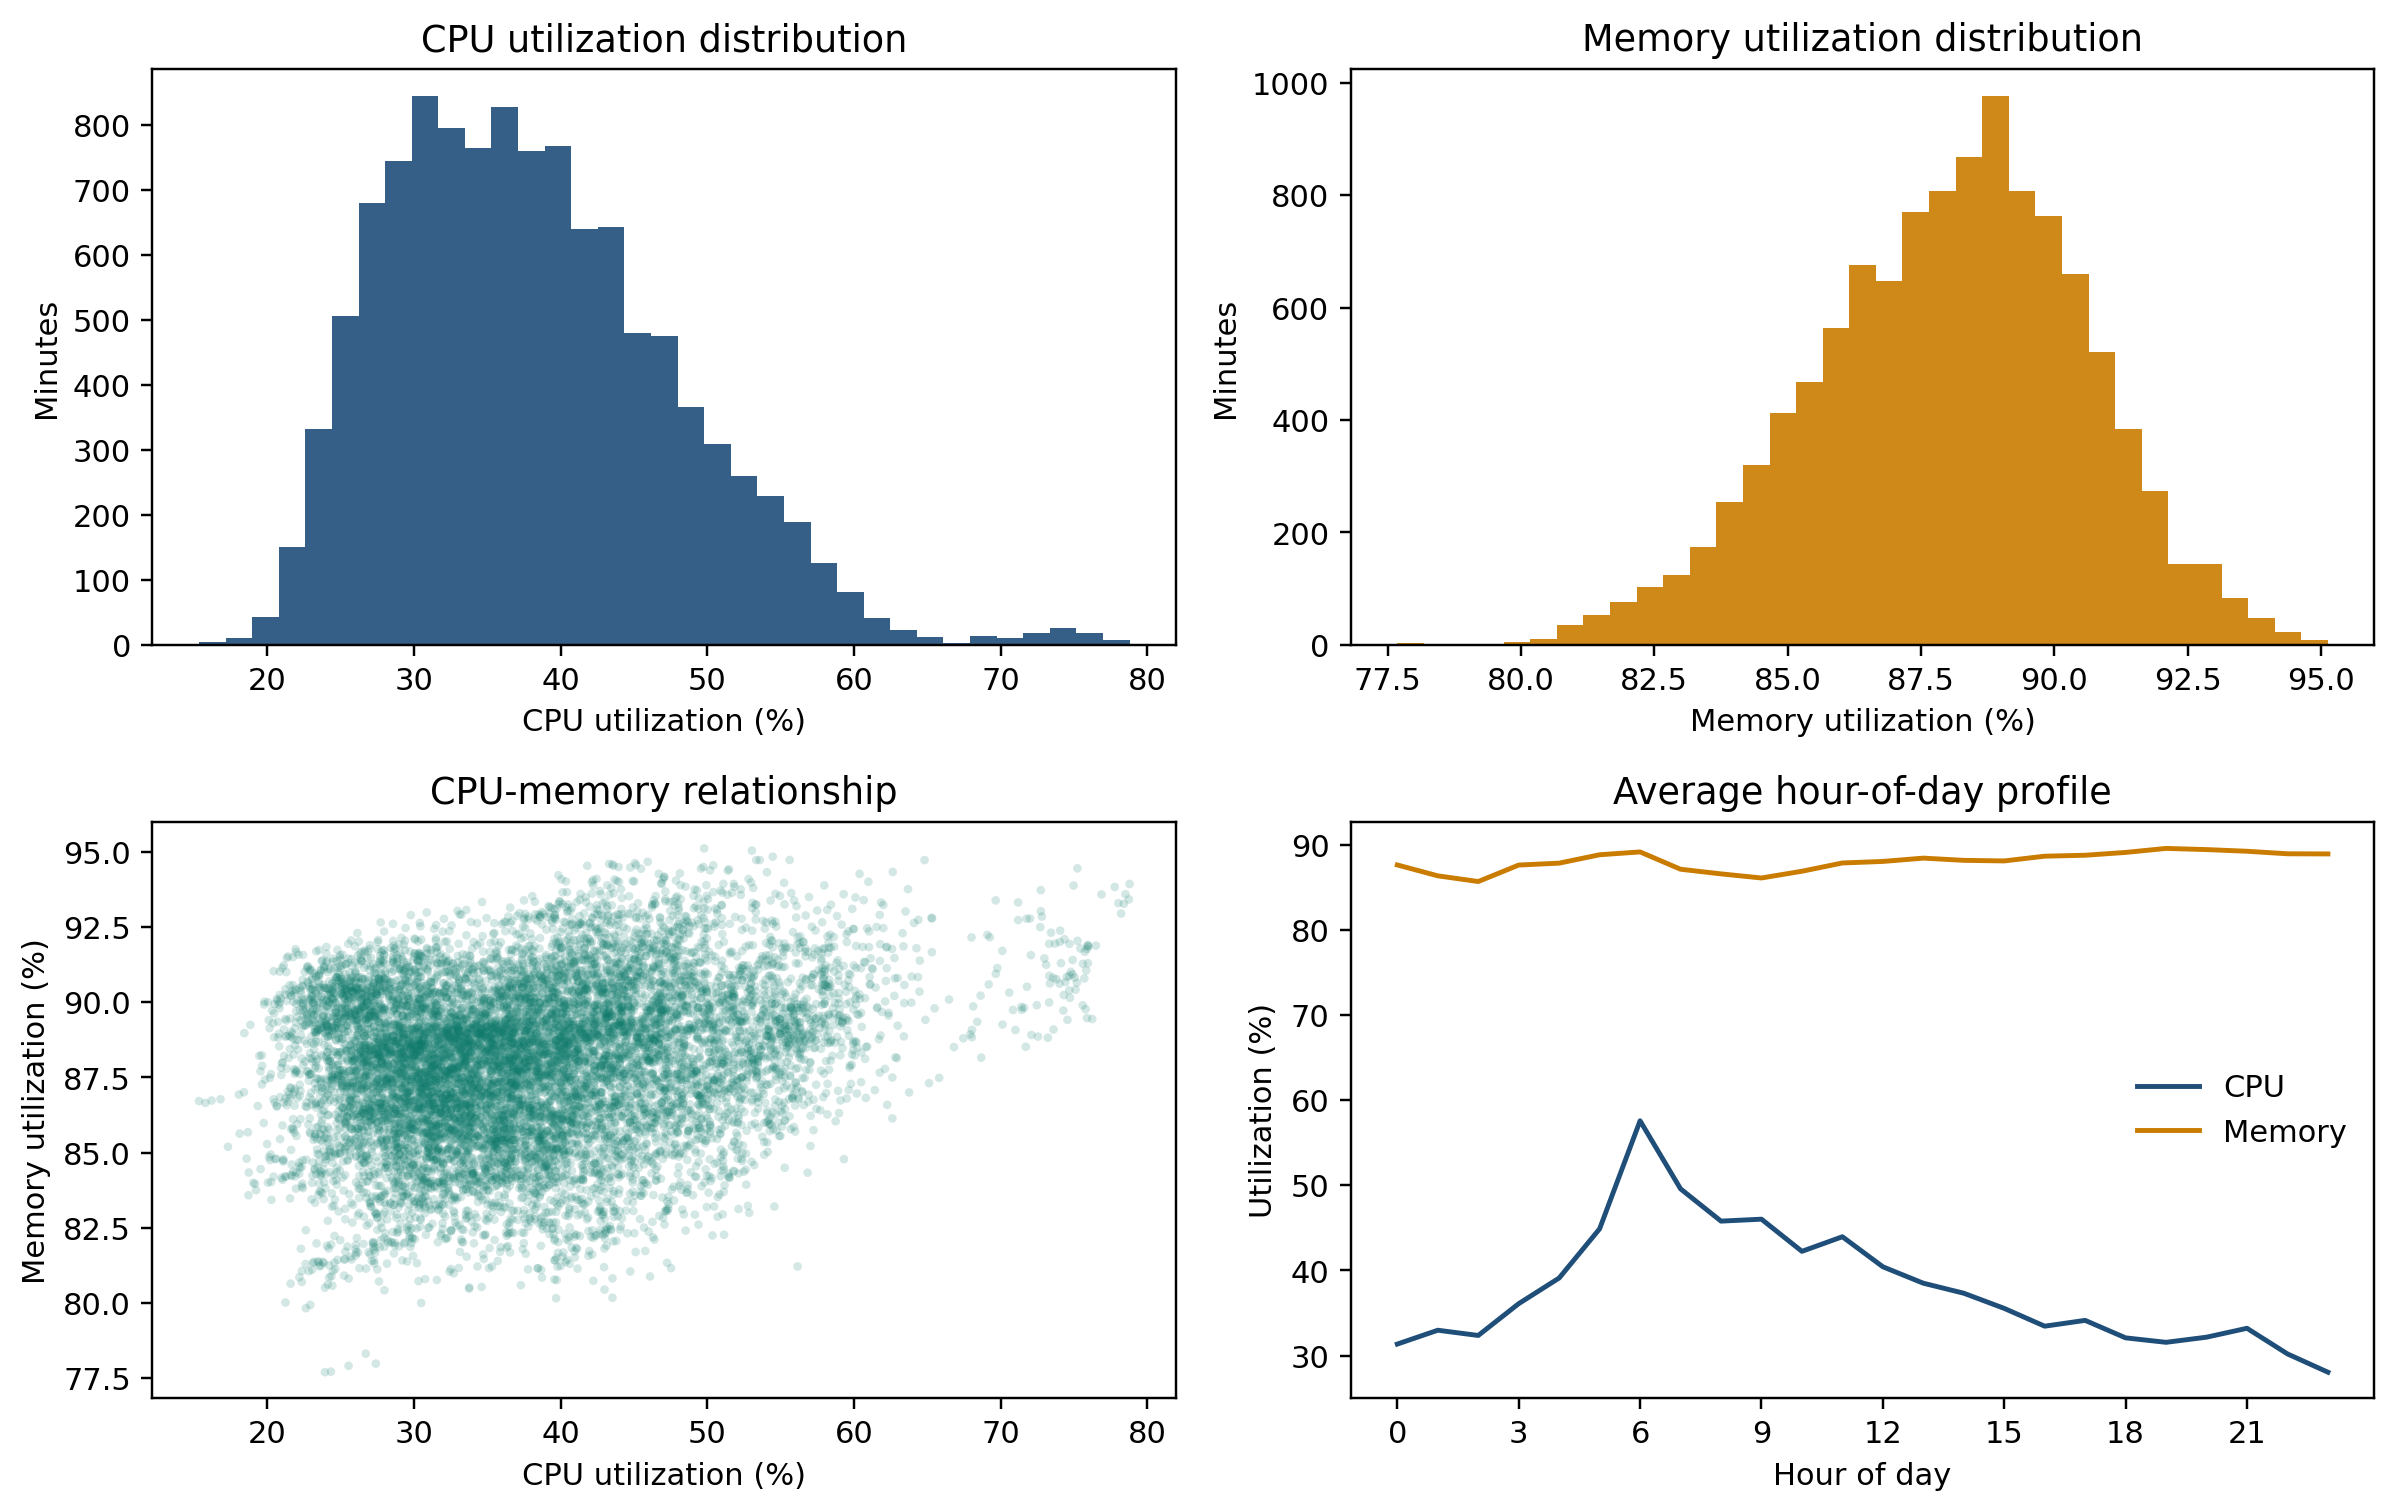
\includegraphics[width=\linewidth]{../experiments/results/figures/resource_distribution_views.png}
  \caption{Additional views of the processed series: CPU distribution, memory distribution, CPU-memory relationship, and average hour-of-day profile.}
  \label{fig:distribution-views}
\end{figure}

\begin{figure}[htbp]
  \centering
  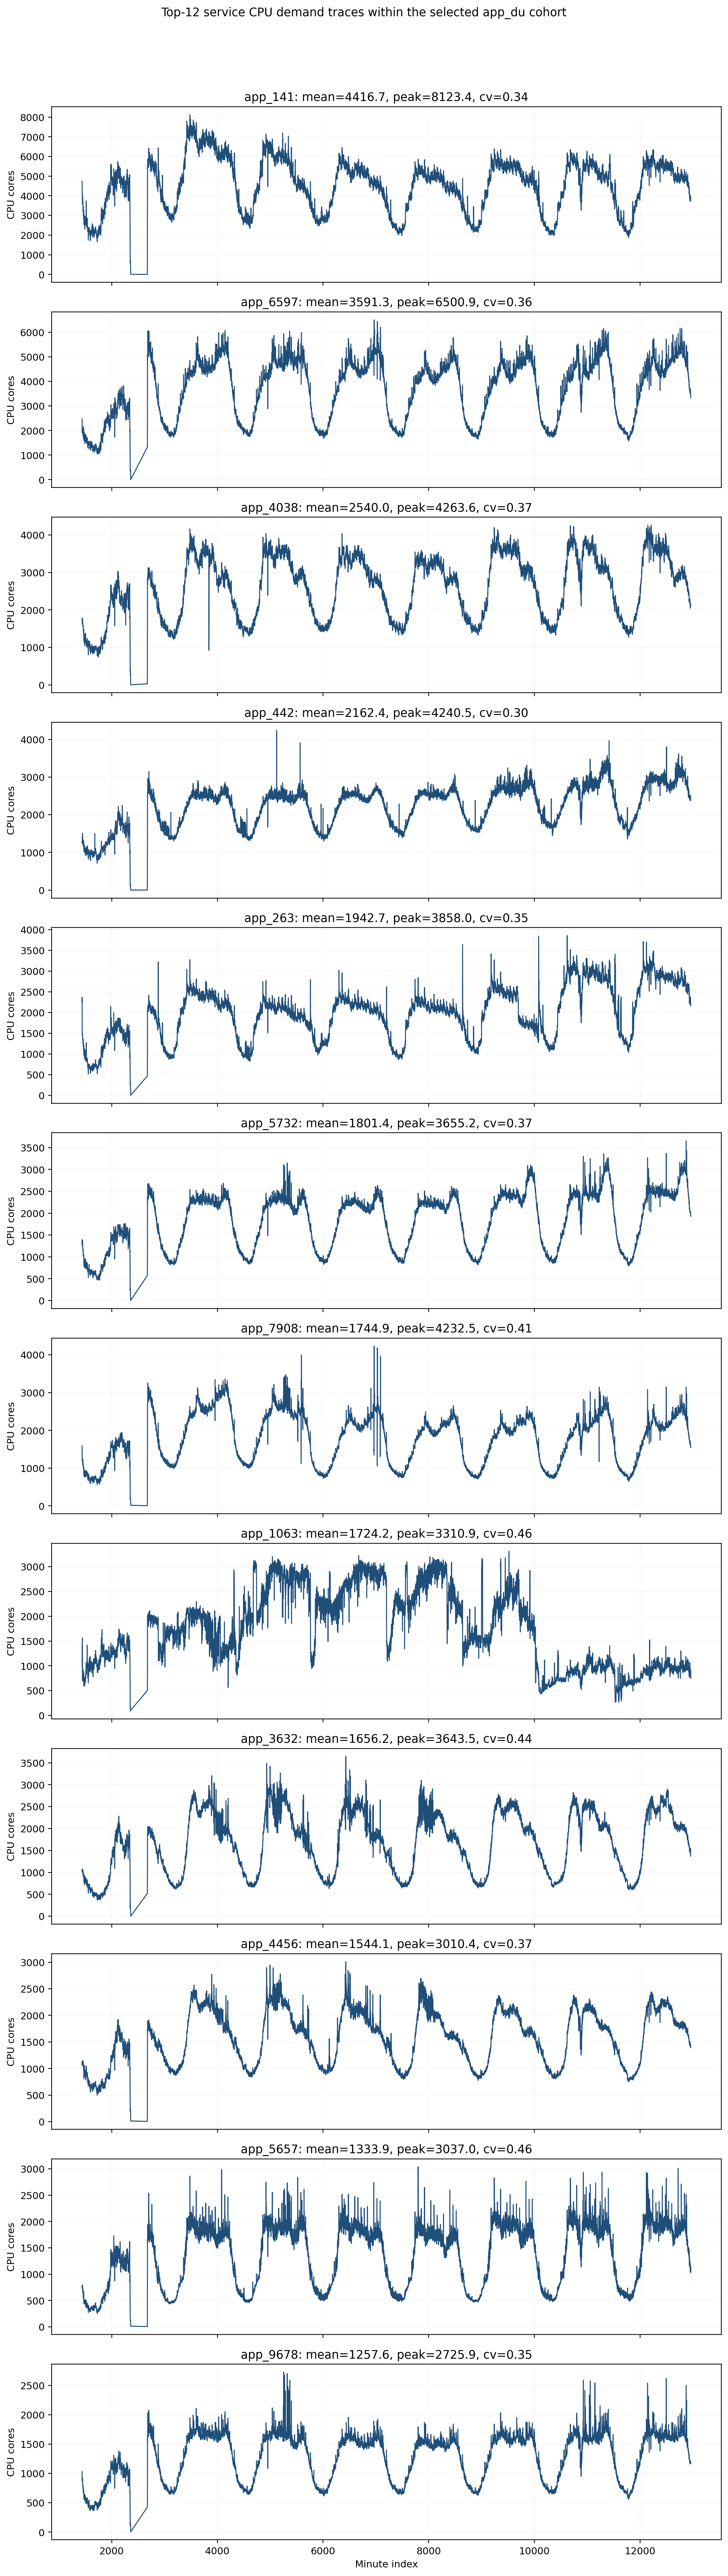
\includegraphics[width=0.78\linewidth]{../experiments/results/service_cohort_broad/figures/service_workload_overview.png}
  \caption{Twelve representative high-demand services from the broad \texttt{app\_du} cohort. Even under the same shared minute span, the retained services differ markedly in mean load, smoothness, and burstiness.}
  \label{fig:service-workload-overview}
\end{figure}

\subsection{Forecasting and policy configuration}

The forecasting benchmark currently implements five point-forecast baselines: persistence, moving average, linear regression, random forest, and a standard feed-forward multilayer perceptron (MLP) regressor. In addition, it implements \texttt{UA-MSTCN-Lite}, a trainable uncertainty-aware surrogate that uses multi-scale history features together with a quantile-aware tree ensemble. The MLP is included as a conventional neural baseline that does not assume a specialized temporal architecture. These models serve two roles. First, they validate the experiment harness without requiring a heavyweight sequence-model stack. Second, they define increasingly strong performance floors that a later deep TCN variant must exceed.

The aggregate series is split chronologically into training, validation, and test segments using a $70/15/15$ partition. The training route consumes the first 85\% of the series, and the test route consumes the final 15\% only; all forecasting numbers reported in this revision use this leakage-free split. The context window is fixed to 60 minutes in the default configuration, and forecast horizons are set to 1, 5, and 10 minutes. This choice balances operational relevance with manageable control lag. Forecasting quality is measured with MAE, RMSE, MAPE, and pinball loss.

The autoscaling simulator compares three policies:
\begin{enumerate}
  \item a reactive threshold policy with upper and lower utilization thresholds, and
  \item a lagged target-tracking policy that follows the previous-step required capacity under the same step-size constraint, and
  \item a predictive policy that uses median and high-quantile forecasts with cooldown and maximum-step constraints.
\end{enumerate}
All three policies act on a normalized aggregate capacity signal. The predictive route uses the calibrated high-quantile forecast for scale-out, adds the configured scale-out margin, and evaluates decisions in the same required-capacity space as the reactive and lagged baselines.

\subsection{Extended analysis protocol}

Beyond the core benchmark tables, the protocol includes six additional analyses:
\begin{enumerate}
  \item \textbf{Context sensitivity:} the \texttt{UA-MSTCN-Lite} context window is varied over 30, 60, and 120 minutes to test short- versus long-history dependence.
  \item \textbf{Regime analysis:} the 5-minute horizon test windows are partitioned into stable, moderate, and bursty subsets according to the local standard deviation of the recent 30-minute history.
  \item \textbf{Quantile calibration:} empirical $P50$ and $P90$ coverage, together with interval width, are measured for the uncertainty-aware surrogate.
  \item \textbf{Policy ablation and sensitivity:} the predictive controller is re-evaluated after removing the scale-out margin, removing cooldown, collapsing to median-only forecasts, and sweeping the scale-out margin/cooldown pair.
  \item \textbf{Cross-machine transfer:} pooled global models are trained on 8 machines and evaluated zero-shot on 4 held-out machines, repeated over 3 deterministic folds.
  \item \textbf{Service-level evidence:} a rule-based broad \texttt{app\_du} cohort extracted from official container tables is used to test both forecast calibration and predictive control at a more natural autoscaling unit.
\end{enumerate}
For the service-level policy route, the protocol fixes the resampling unit to \texttt{service}. The primary comparison statistic is the equal-weighted mean predictive-minus-reactive delta across retained services, while a load-weighted mean delta using the service CPU-cores proxy is reported only as an auxiliary sensitivity check. Stability is assessed with paired bootstrap over services using a fixed resample count and the following interpretation rule for lower-is-better metrics: a 95\% interval fully below zero indicates stable improvement, a 95\% interval fully above zero indicates stable degradation, and an interval that crosses zero is treated as not stable. The same pre-fixed rule also governs service-cohort promotion: a broader audited cohort replaces the earlier targeted mainline if the forecasting headline flips, if a policy headline mean direction flips, or if an earlier declarative gain on service-level over-provisioning or scaling actions is no longer stably supportable.
For the machine cohort, the same leakage-free forecasting setup is reused so that aggregate and cross-entity results remain directly comparable.

\subsection{Artifacts and environment}

The experimental pipeline writes its outputs to \texttt{paper-workbench/experiments/results/}. The metrics contract is fixed by \texttt{metrics.csv}, the policy time series is exported as \texttt{policy\_series.csv}, and the manuscript figures are rendered from these artifacts rather than edited manually. This contract is important because the manuscript should consume experiment outputs directly rather than rely on hand-copied numbers.

The experiments were executed with TeX Live 2023, \texttt{pdflatex}, and \texttt{latexmk} for manuscript compilation, together with a dedicated Python environment containing \texttt{pandas}, \texttt{scikit-learn}, \texttt{pyyaml}, and \texttt{matplotlib}. This keeps the current implementation lightweight and reproducible.


\section{Results and Discussion}
The manuscript now reports leakage-free forecasting results, uncertainty-calibration checks, cross-entity transfer checks, broad service-level evidence from official container traces, and a calibrated control comparison based on a trainable uncertainty-aware surrogate. The evidence is strong enough for a multi-granularity discussion, while still leaving room for service-aware tuning and stronger deep temporal models.

\subsection{Forecasting benchmark}

The experimental pipeline includes a reproducible downloader for Alibaba \texttt{v2018} artifacts, a preprocessing route that builds a one-minute aggregate workload series from the compressed trace, baseline forecasters, a trainable \texttt{UA-MSTCN-Lite} surrogate, and a predictive-versus-reactive policy simulator. Most importantly, the reported metrics are computed on 11{,}208 aggregate samples rather than on placeholder values.

Table~\ref{tab:forecast-smoke-test} summarizes aggregate forecasting results under the leakage-free split. Linear regression provides the best average MAE across the three horizons (3.514), random forest is a close second (3.529), and \texttt{UA-MSTCN-Lite} remains competitive rather than dominant (3.548 average MAE). The standard neural MLP baseline improves over persistence and moving average, but its average MAE of 3.708 does not overturn the linear-tree ranking. At the 10-minute horizon, the gap between linear regression and \texttt{UA-MSTCN-Lite} is only 0.0013 MAE, which is small enough to treat the two models as practically tied on this aggregate signal. The aggregate benchmark therefore shows that the uncertainty-aware surrogate can still support the control study even when it is not the strongest point forecaster.

\begin{table}[htbp]
  \centering
  \caption{Verified smoke-test forecasting performance on the aggregate cluster series.}
  \label{tab:forecast-smoke-test}
  \scriptsize
  \setlength{\tabcolsep}{2pt}
  \renewcommand{\arraystretch}{0.96}
  \begin{tabular}{lcccc}
    \toprule
    Model & Horizon & MAE & RMSE & MAPE \\
    \midrule
    Persistence & 1 & 2.395 & 3.285 & 0.060 \\
    Moving average & 1 & 3.215 & 4.348 & 0.079 \\
    Linear regression & 1 & 2.268 & 3.123 & 0.056 \\
    Random forest & 1 & 2.324 & 3.176 & 0.058 \\
    MLP regressor & 1 & 2.422 & 3.267 & 0.061 \\
    UA-MSTCN-Lite & 1 & 2.349 & 3.214 & 0.058 \\
    Persistence & 5 & 4.569 & 6.162 & 0.112 \\
    Moving average & 5 & 4.387 & 5.850 & 0.107 \\
    Linear regression & 5 & 3.967 & 5.324 & 0.098 \\
    Random forest & 5 & 3.928 & 5.237 & 0.097 \\
    MLP regressor & 5 & 4.276 & 5.603 & 0.105 \\
    UA-MSTCN-Lite & 5 & 3.986 & 5.304 & 0.098 \\
    Persistence & 10 & 5.119 & 6.785 & 0.126 \\
    Moving average & 10 & 4.845 & 6.409 & 0.119 \\
    Linear regression & 10 & 4.307 & 5.765 & 0.107 \\
    Random forest & 10 & 4.334 & 5.780 & 0.107 \\
    MLP regressor & 10 & 4.427 & 5.781 & 0.109 \\
    UA-MSTCN-Lite & 10 & 4.308 & 5.793 & 0.107 \\
    \bottomrule
  \end{tabular}
\end{table}

\begin{figure}[htbp]
  \centering
  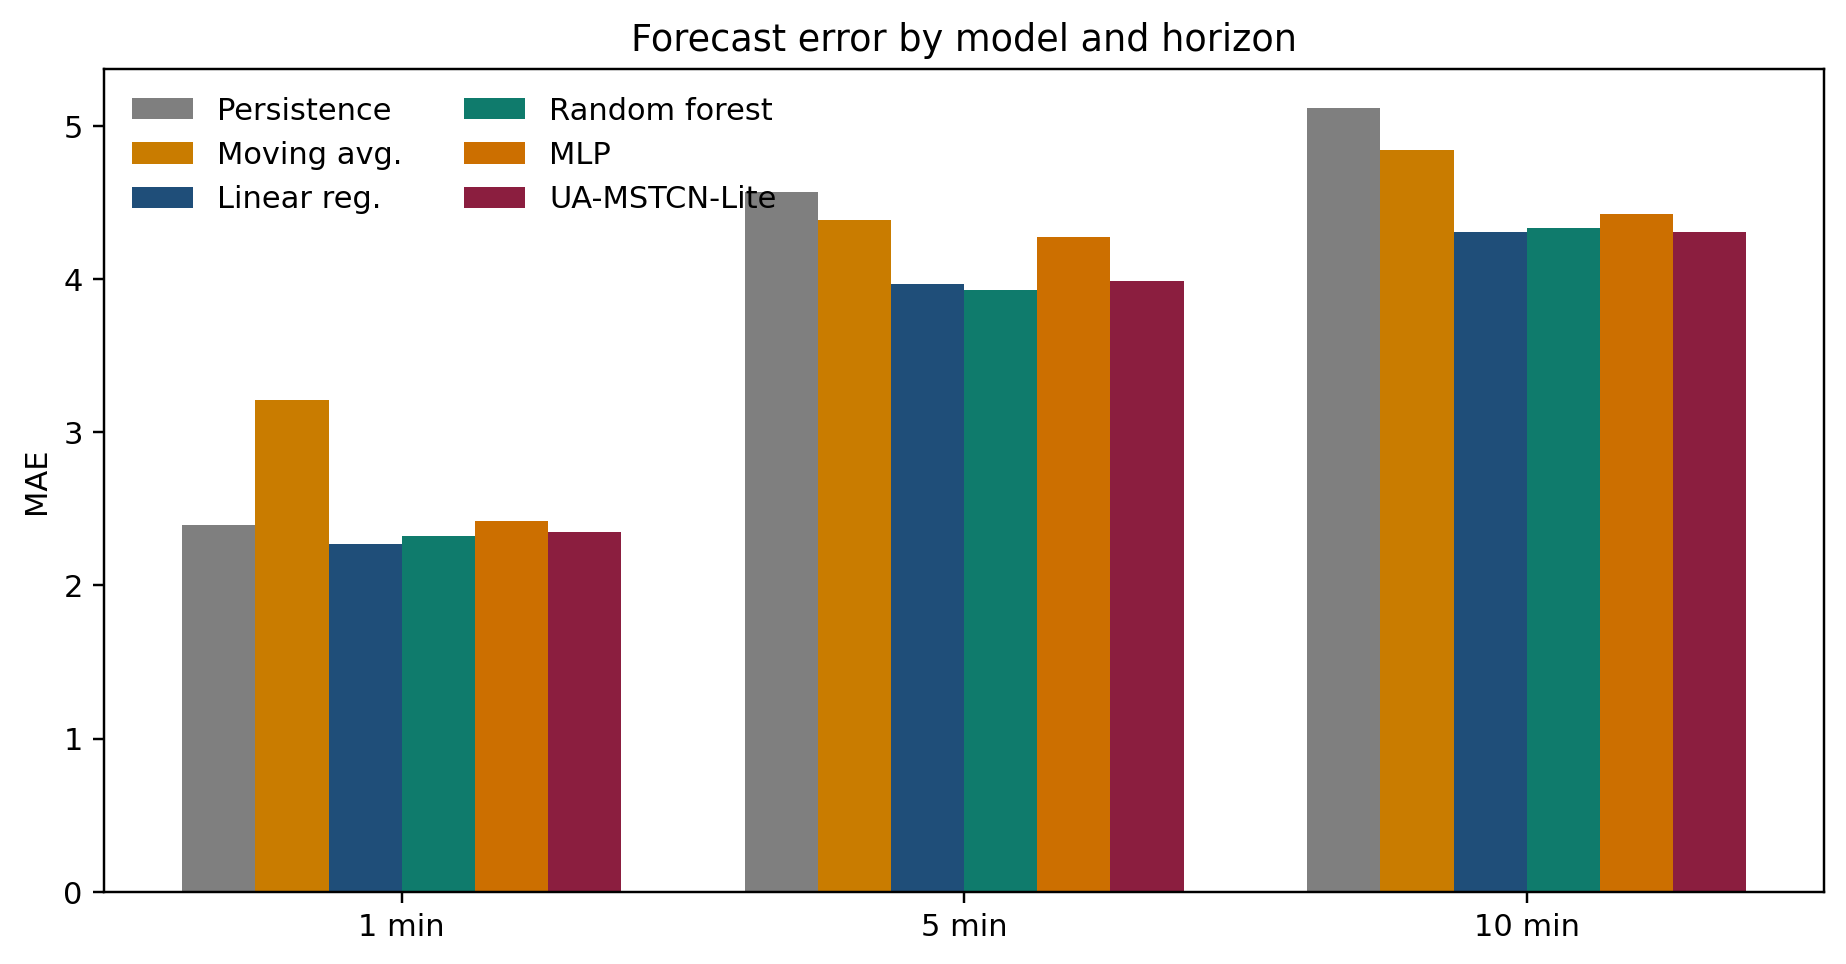
\includegraphics[width=\linewidth]{../experiments/results/figures/baseline_mae_by_horizon.png}
  \caption{Forecast error by model and horizon after the leakage-free split correction. Linear regression remains the strongest average point forecaster, while the standard neural MLP baseline improves over simple heuristics without changing the overall ranking.}
  \label{fig:mae-by-horizon}
\end{figure}

\subsection{Case study and accuracy-runtime trade-off}

Aggregate error tables alone do not show where the models succeed or fail. Figure~\ref{fig:forecast-case-study} therefore plots aligned slices from the test set at the 1-, 5-, and 10-minute horizons. The same pattern appears across horizons: persistence reacts too slowly when the workload turns, the MLP captures the broad trend but remains smoother around turning points, and random forest together with \texttt{UA-MSTCN-Lite} tracks the main shape more closely. The figure is still useful even though \texttt{UA-MSTCN-Lite} is no longer the best average point forecaster, because the controller consumes its quantile band rather than only its median prediction.

\begin{figure}[htbp]
  \centering
  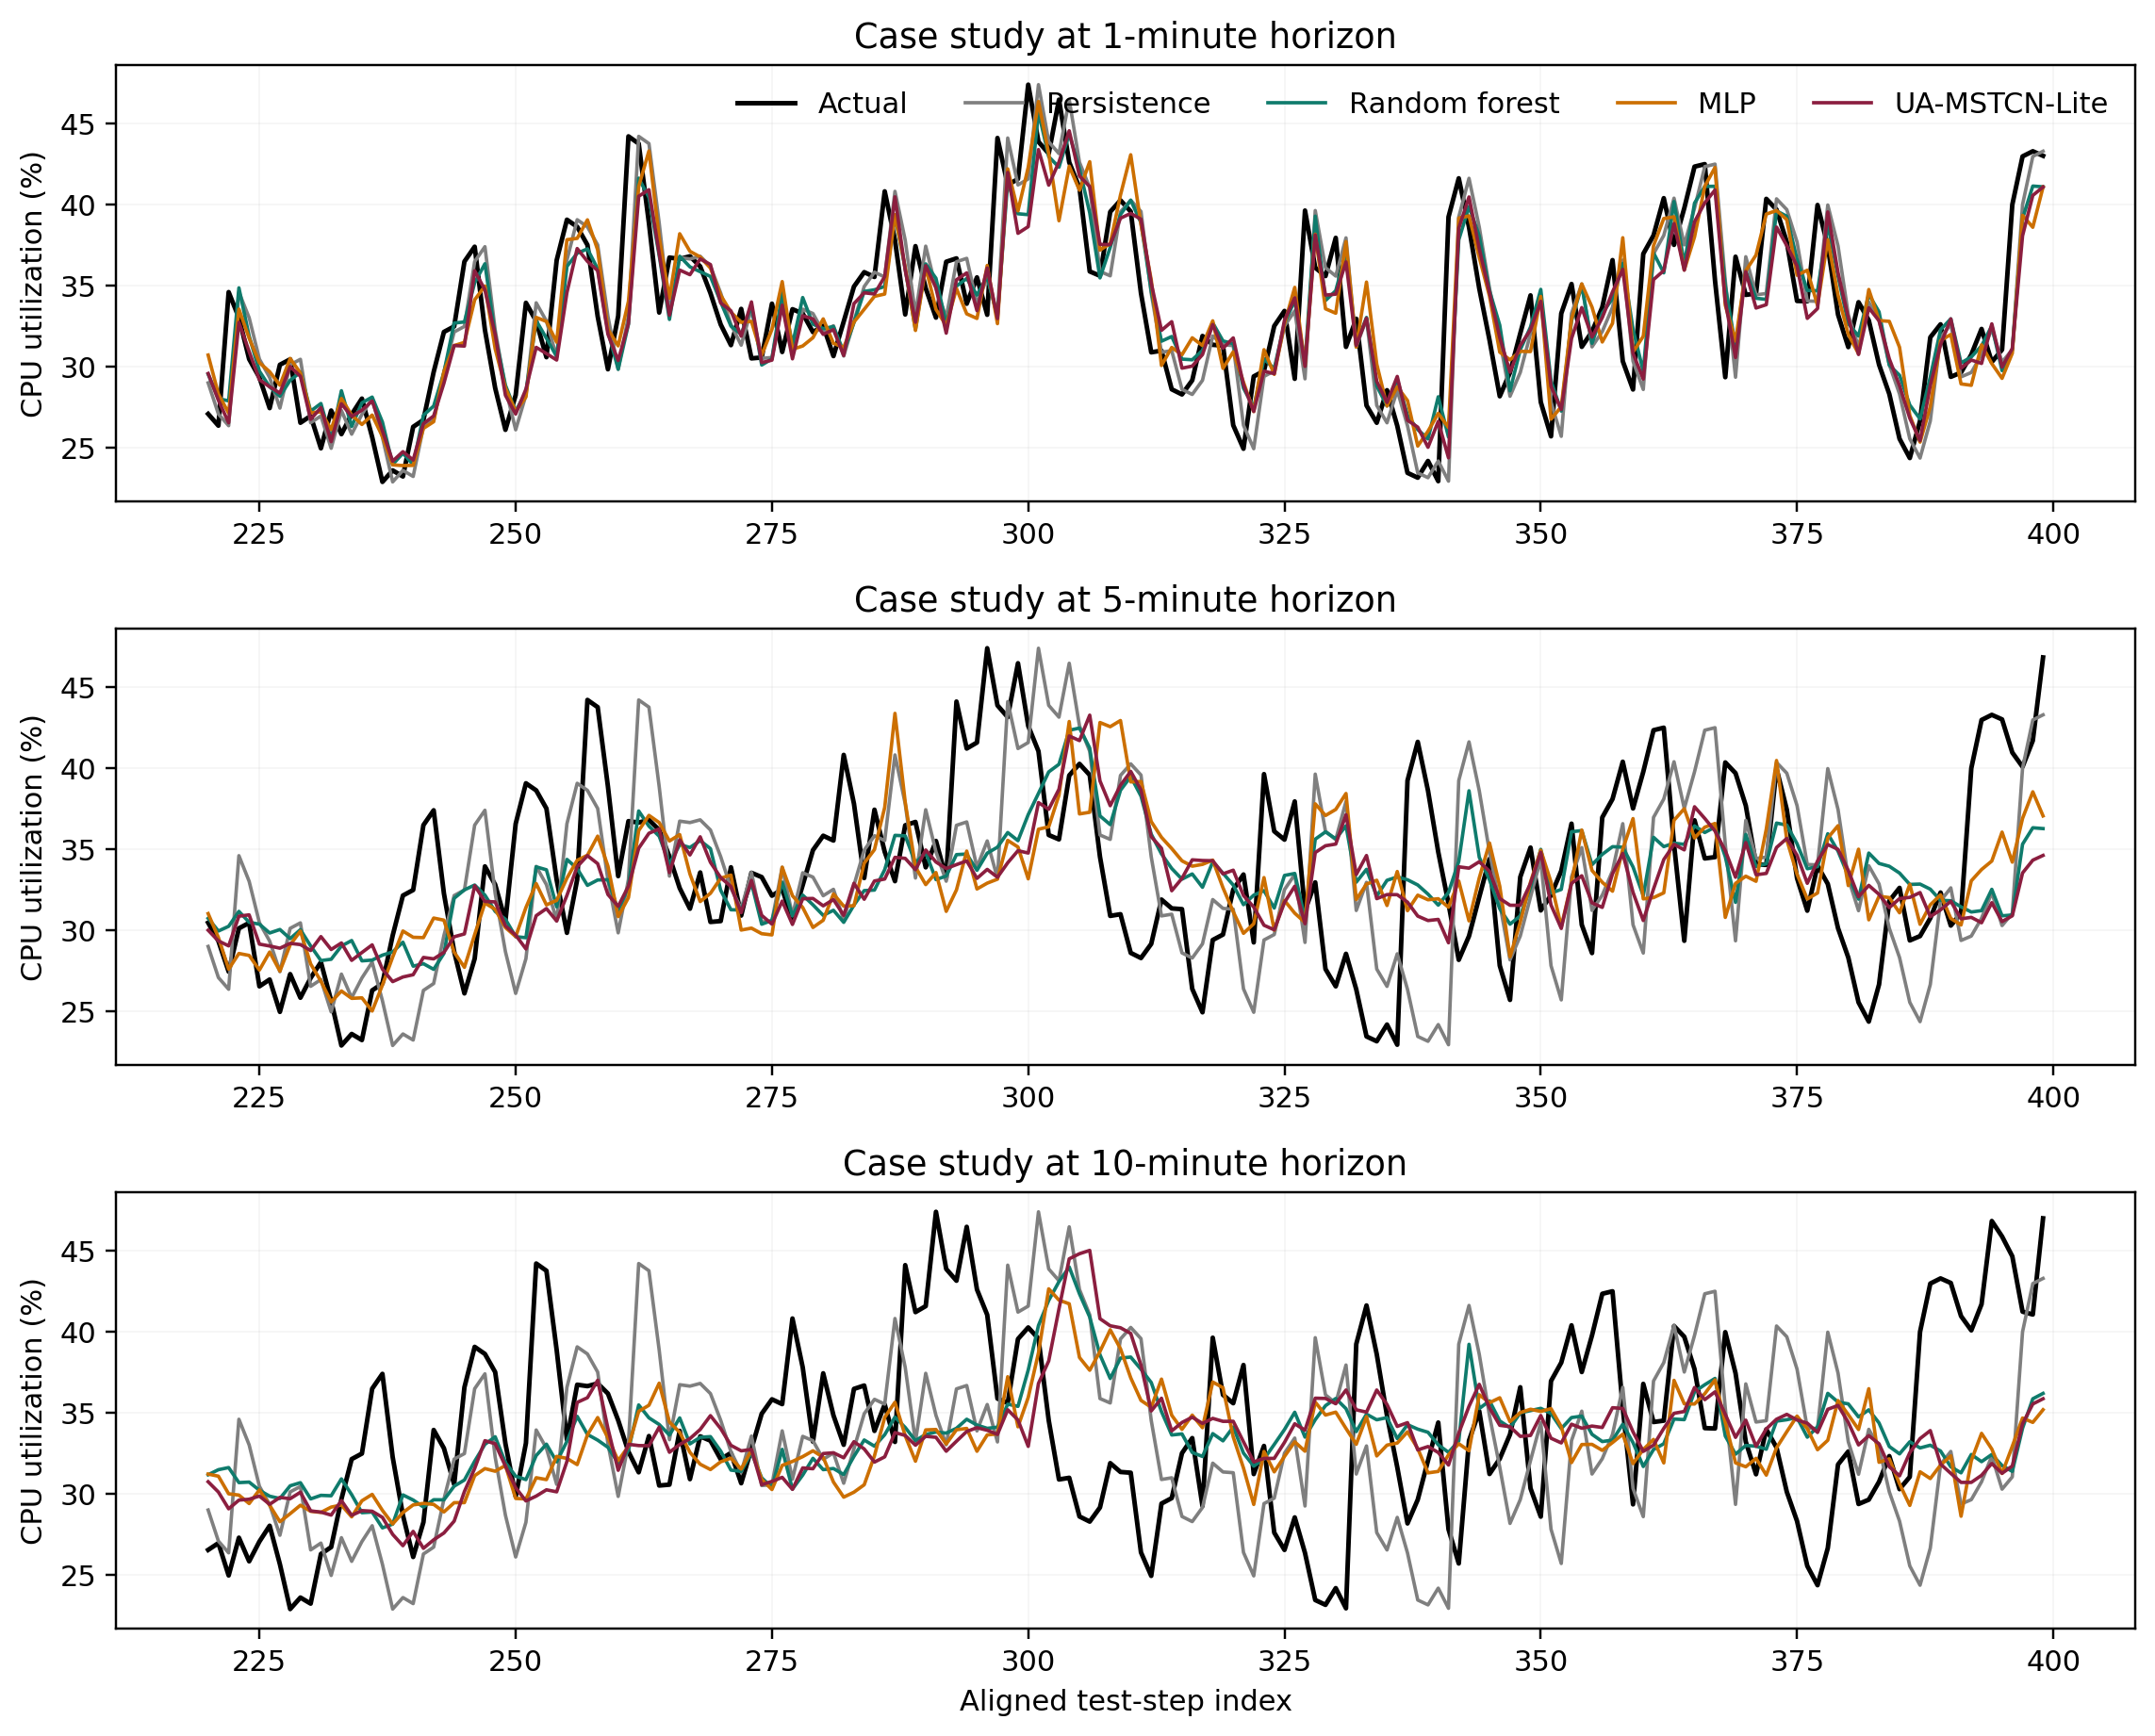
\includegraphics[width=\linewidth]{../experiments/results/figures/forecast_case_study.png}
  \caption{Forecast case study on aligned test slices for the 1-, 5-, and 10-minute horizons.}
  \label{fig:forecast-case-study}
\end{figure}

Accuracy is not the only practical concern. Figure~\ref{fig:latency-tradeoff} shows the trade-off between average MAE and average wall-clock runtime per benchmark call on the current workstation. Linear regression is now the strongest average point predictor at 19.3 ms per benchmark call, the MLP baseline sits in the middle at about 630 ms per call, random forest is slightly better in MAE than MLP but over an order of magnitude slower, and \texttt{UA-MSTCN-Lite} stays close to random forest in average MAE while also producing calibrated uncertainty estimates. This observation matters because it separates two questions that are often conflated: which model is best for point forecasting, and which model exposes the uncertainty information needed by the controller.

\begin{figure}[htbp]
  \centering
  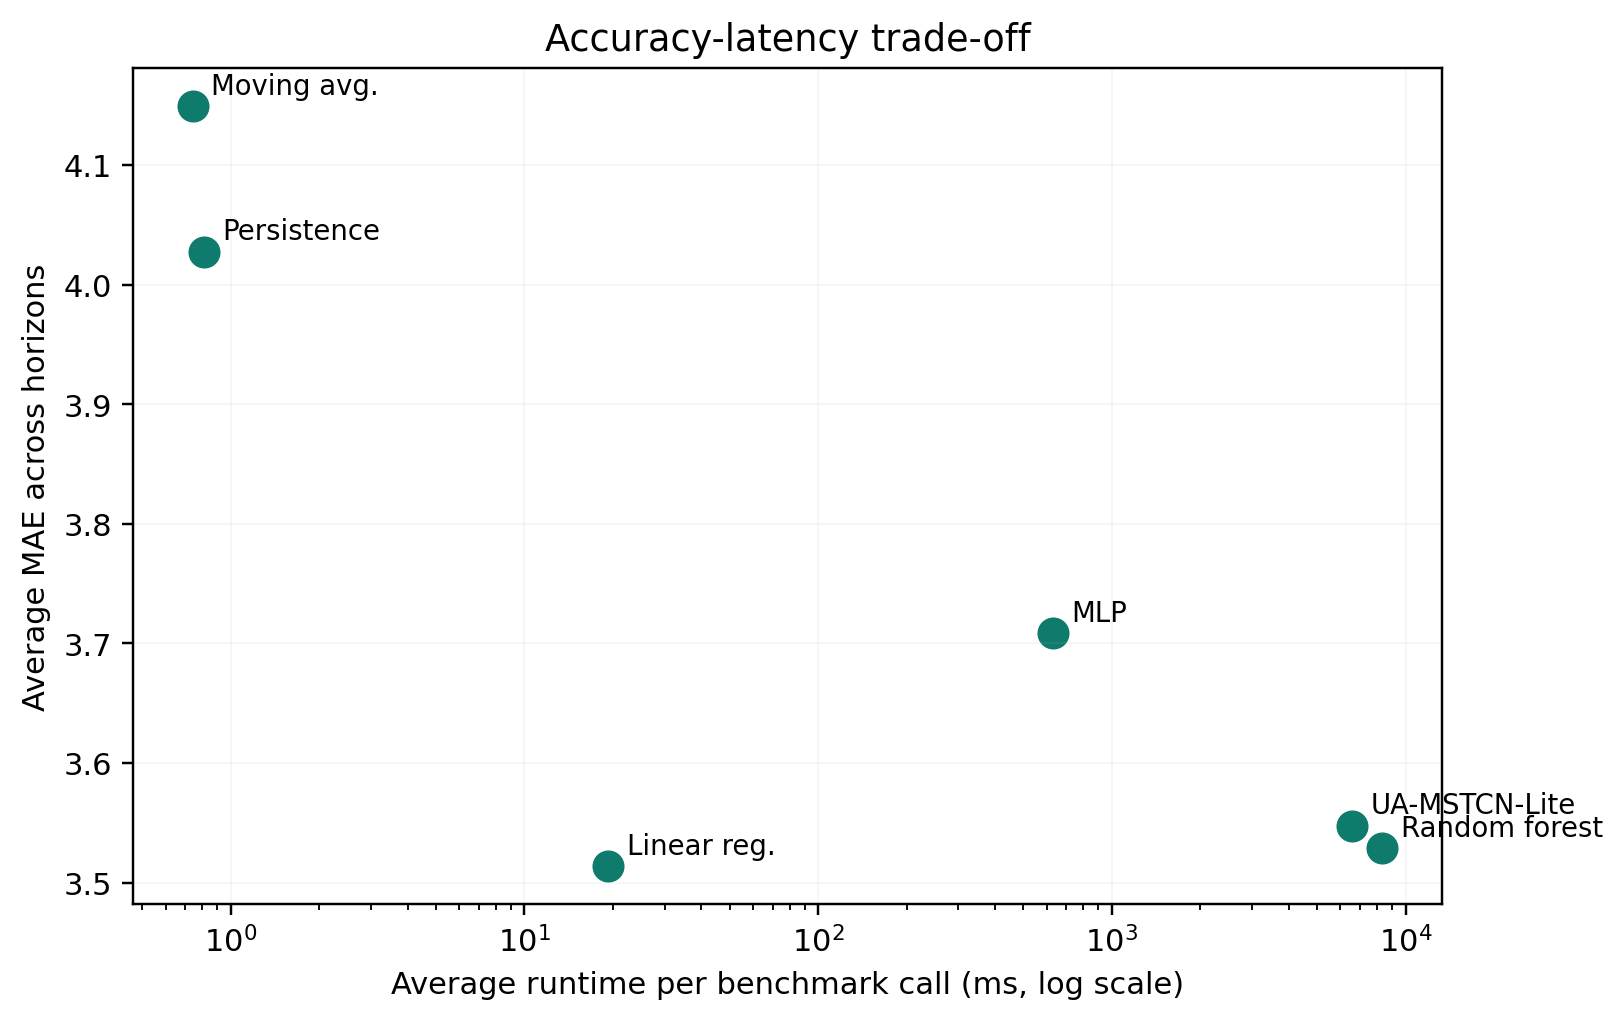
\includegraphics[width=0.82\linewidth]{../experiments/results/figures/forecast_latency_tradeoff.png}
  \caption{Average forecasting accuracy versus average runtime per benchmark call on the current workstation.}
  \label{fig:latency-tradeoff}
\end{figure}

\subsection{Context, regime, and calibration analysis}

The aggregate route also includes three forecasting diagnostics. First, Figure~\ref{fig:context-sensitivity} shows the sensitivity of \texttt{UA-MSTCN-Lite} to the context window. A 60-minute window gives the best average MAE (3.548), compared with 3.615 for 30 minutes and 3.585 for 120 minutes. The result is modest rather than dramatic, but it is still useful because it shows the default context length is not arbitrary.

\begin{figure}[htbp]
  \centering
  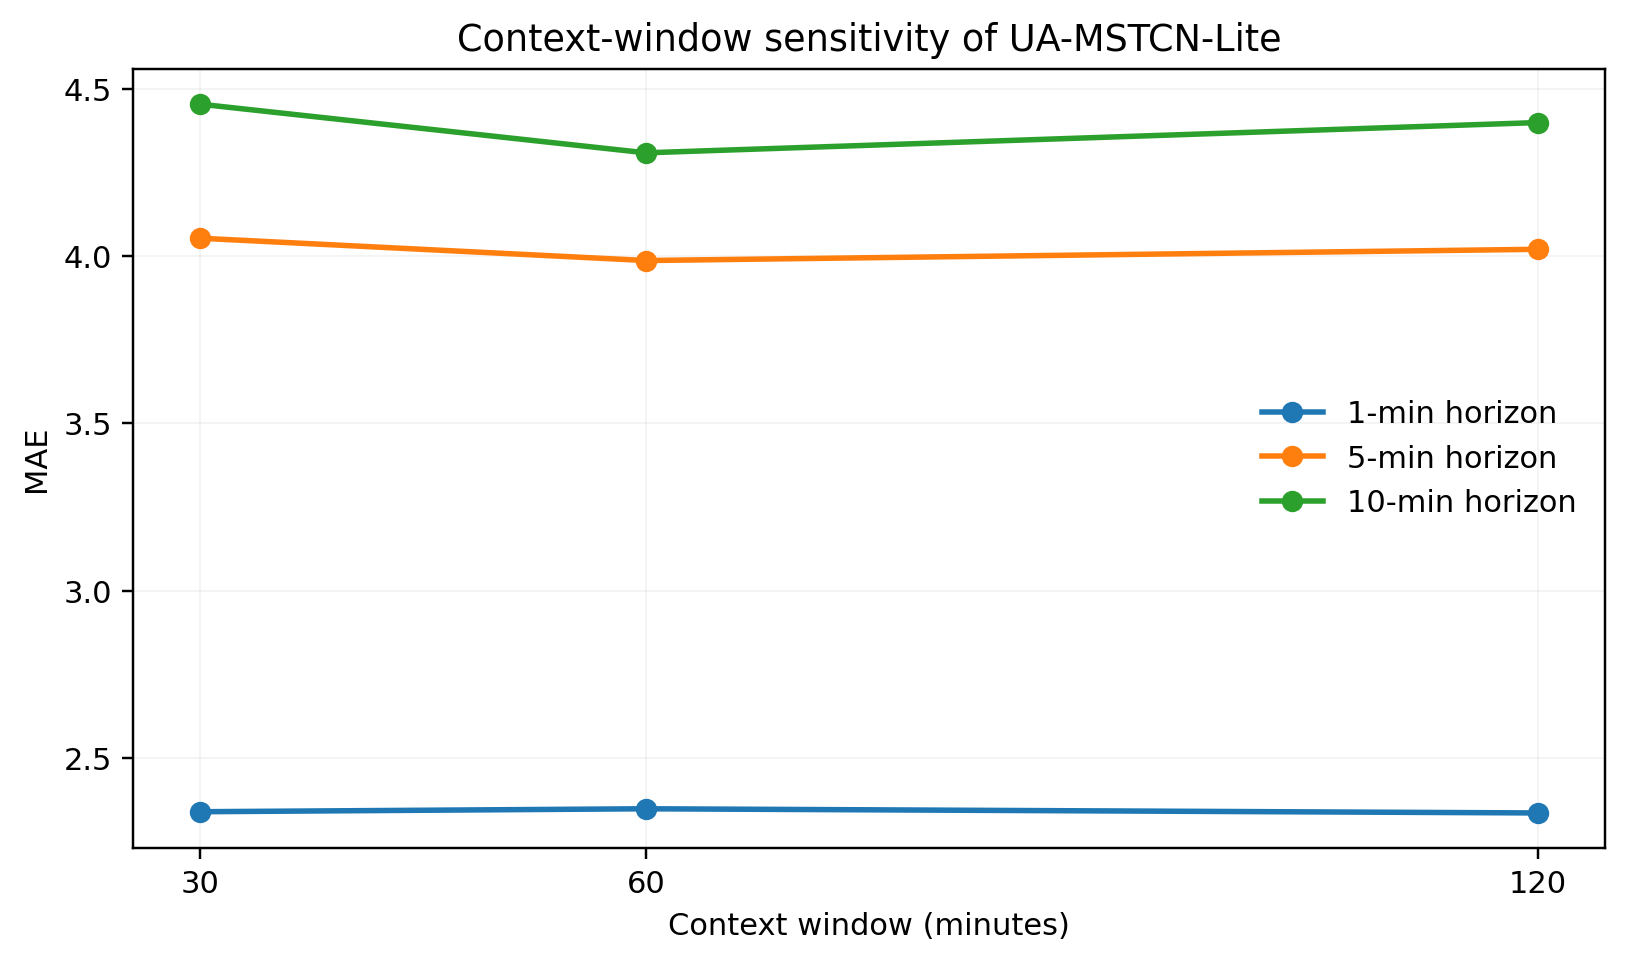
\includegraphics[width=0.76\linewidth]{../experiments/results/figures/ua_context_sensitivity.png}
  \caption{Context-window sensitivity of \texttt{UA-MSTCN-Lite}. The 60-minute default gives the best average MAE across the three evaluation horizons.}
  \label{fig:context-sensitivity}
\end{figure}

Second, Figure~\ref{fig:regime-comparison} partitions the 5-minute horizon test set into stable, moderate, and bursty regimes according to recent local volatility. The result again argues for caution rather than overclaiming: \texttt{UA-MSTCN-Lite} is slightly better than random forest in the moderate regime (3.731 vs.\ 3.752 MAE), but slightly worse in the stable and bursty regimes. This regime split shows that the surrogate is not hiding a brittle failure mode behind a single mean score, and it identifies bursty demand as the regime that most clearly needs a stronger next-generation model.

\begin{figure}[htbp]
  \centering
  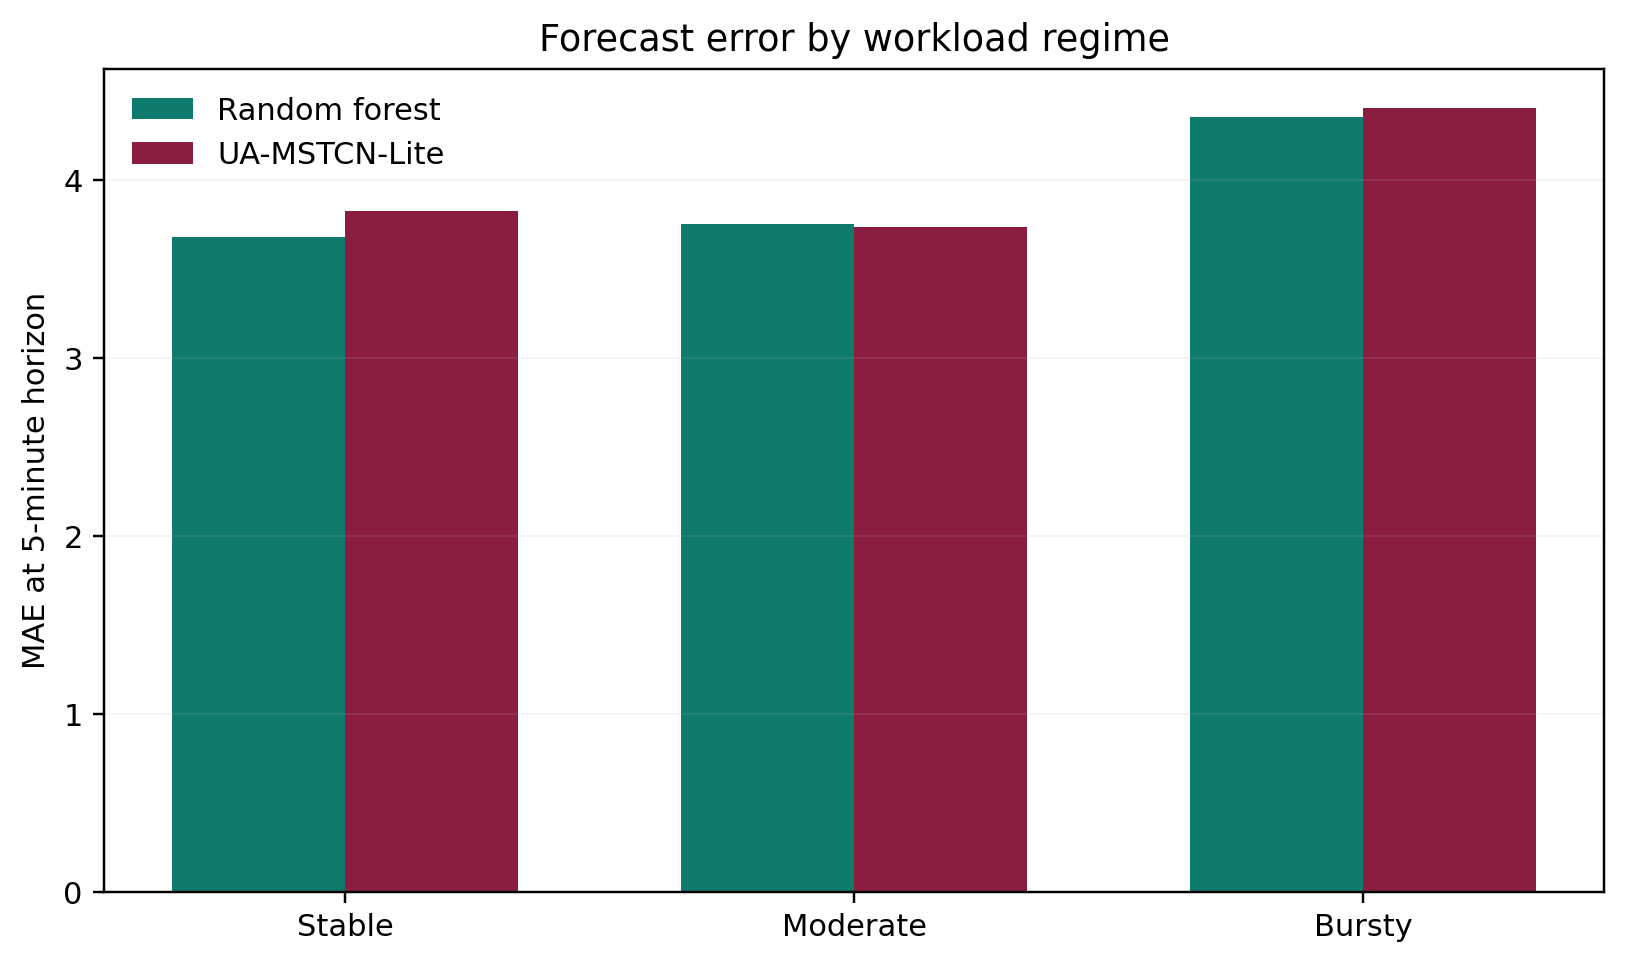
\includegraphics[width=0.76\linewidth]{../experiments/results/figures/forecast_regime_comparison.png}
  \caption{Forecast error at the 5-minute horizon across stable, moderate, and bursty workload regimes.}
  \label{fig:regime-comparison}
\end{figure}

Third, the uncertainty-aware surrogate is now evaluated directly through empirical quantile coverage. Table~\ref{tab:quantile-coverage} and Figure~\ref{fig:quantile-coverage} show that the median forecasts are well centered, with $P50$ coverage staying close to 0.5 across all horizons. The high quantile is slightly conservative at the 1-minute horizon (0.920 coverage) and mildly under-covered at the 5- and 10-minute horizons (0.867 and 0.868). This is a useful control-oriented result: the quantile band is credible enough to support a predictive policy, but the longer-horizon under-coverage explains why the controller still needs an explicit scale-out margin.

\begin{table}[htbp]
  \centering
  \caption{Empirical quantile coverage of \texttt{UA-MSTCN-Lite} on the aggregate test split.}
  \label{tab:quantile-coverage}
  \scriptsize
  \setlength{\tabcolsep}{3pt}
  \renewcommand{\arraystretch}{0.96}
  \begin{tabular}{lccc}
    \toprule
    Horizon & $P50$ cov. & $P90$ cov. & Mean int. width \\
    \midrule
    1 minute & 0.506 & 0.920 & 4.623 \\
    5 minutes & 0.516 & 0.867 & 6.709 \\
    10 minutes & 0.500 & 0.868 & 7.405 \\
    \bottomrule
  \end{tabular}
\end{table}

\begin{figure}[htbp]
  \centering
  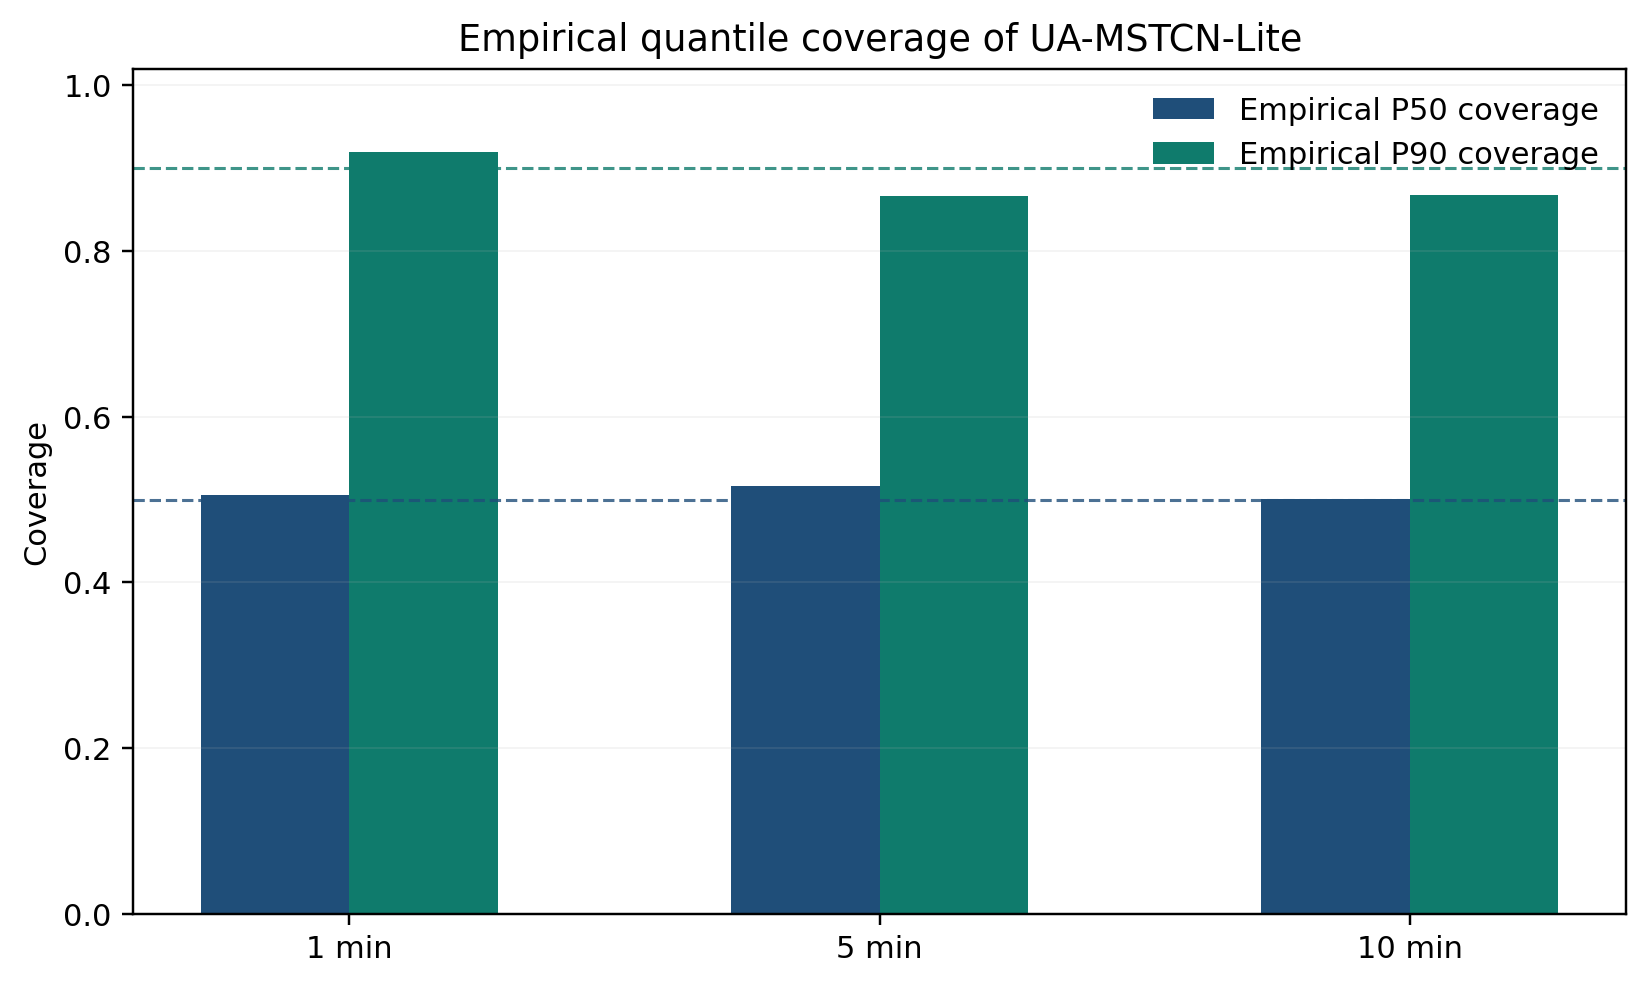
\includegraphics[width=0.72\linewidth]{../experiments/results/figures/quantile_coverage.png}
  \caption{Empirical $P50$ and $P90$ coverage of \texttt{UA-MSTCN-Lite}. Dashed lines indicate the nominal target levels.}
  \label{fig:quantile-coverage}
\end{figure}

\subsection{Cross-entity machine-cohort benchmark}

The aggregate trace is no longer the only evidence surface. A second benchmark extracted from 12 high-coverage machines tests whether the forecasting story changes once the unit of analysis shifts from one cluster-wide series to multiple long-lived entities. Table~\ref{tab:machine-cohort-summary} summarizes the average error across the cohort. The qualitative ranking is stable and, if anything, harsher on the surrogate than the aggregate benchmark: linear regression is the strongest point predictor at every horizon, with mean MAE values of 3.633, 5.520, and 5.966. The standard neural MLP baseline becomes the second-best average point predictor at all three horizons (3.921, 5.845, and 6.301), but it still trails linear regression by 0.29--0.34 MAE. \texttt{UA-MSTCN-Lite} remains close to random forest and now trails even the simple MLP baseline on this cohort.

\begin{table}[htbp]
  \centering
  \caption{Average forecasting performance across the 12-machine high-coverage cohort.}
  \label{tab:machine-cohort-summary}
  \tiny
  \setlength{\tabcolsep}{2pt}
  \renewcommand{\arraystretch}{0.95}
  \begin{tabular}{lcccc}
    \toprule
    Model & H & MAE & RMSE & MAPE \\
    \midrule
    Persistence & 1 & 3.716 & 5.185 & 0.103 \\
    Linear regression & 1 & 3.633 & 4.926 & 0.101 \\
    MLP regressor & 1 & 3.921 & 5.246 & 0.109 \\
    Random forest & 1 & 4.012 & 5.396 & 0.107 \\
    UA-MSTCN-Lite & 1 & 4.121 & 5.647 & 0.106 \\
    Persistence & 5 & 6.268 & 8.497 & 0.172 \\
    Linear regression & 5 & 5.520 & 7.318 & 0.153 \\
    MLP regressor & 5 & 5.845 & 7.683 & 0.159 \\
    Random forest & 5 & 6.170 & 8.223 & 0.162 \\
    UA-MSTCN-Lite & 5 & 6.244 & 8.423 & 0.161 \\
    Persistence & 10 & 6.932 & 9.390 & 0.192 \\
    Linear regression & 10 & 5.966 & 7.959 & 0.165 \\
    MLP regressor & 10 & 6.301 & 8.324 & 0.172 \\
    Random forest & 10 & 6.548 & 8.745 & 0.173 \\
    UA-MSTCN-Lite & 10 & 6.651 & 8.936 & 0.172 \\
    \bottomrule
  \end{tabular}
\end{table}

Figure~\ref{fig:machine-cohort-mae} makes the same pattern easier to scan. Linear regression wins 6, 8, and 8 of the 12 entities at the 1-, 5-, and 10-minute horizons, respectively. The MLP baseline wins no machine-horizon cell, which shows that its gain over random forest and \texttt{UA-MSTCN-Lite} comes from broad but modest improvements rather than from dominant wins on specific entities. \texttt{UA-MSTCN-Lite} still wins only 2, 3, and 2 entities across these horizons. This is exactly the kind of result that should remain in the manuscript instead of being optimized away: it shows that the current surrogate is not yet the strongest general-purpose point forecaster when the workload granularity becomes finer.

\begin{figure}[htbp]
  \centering
  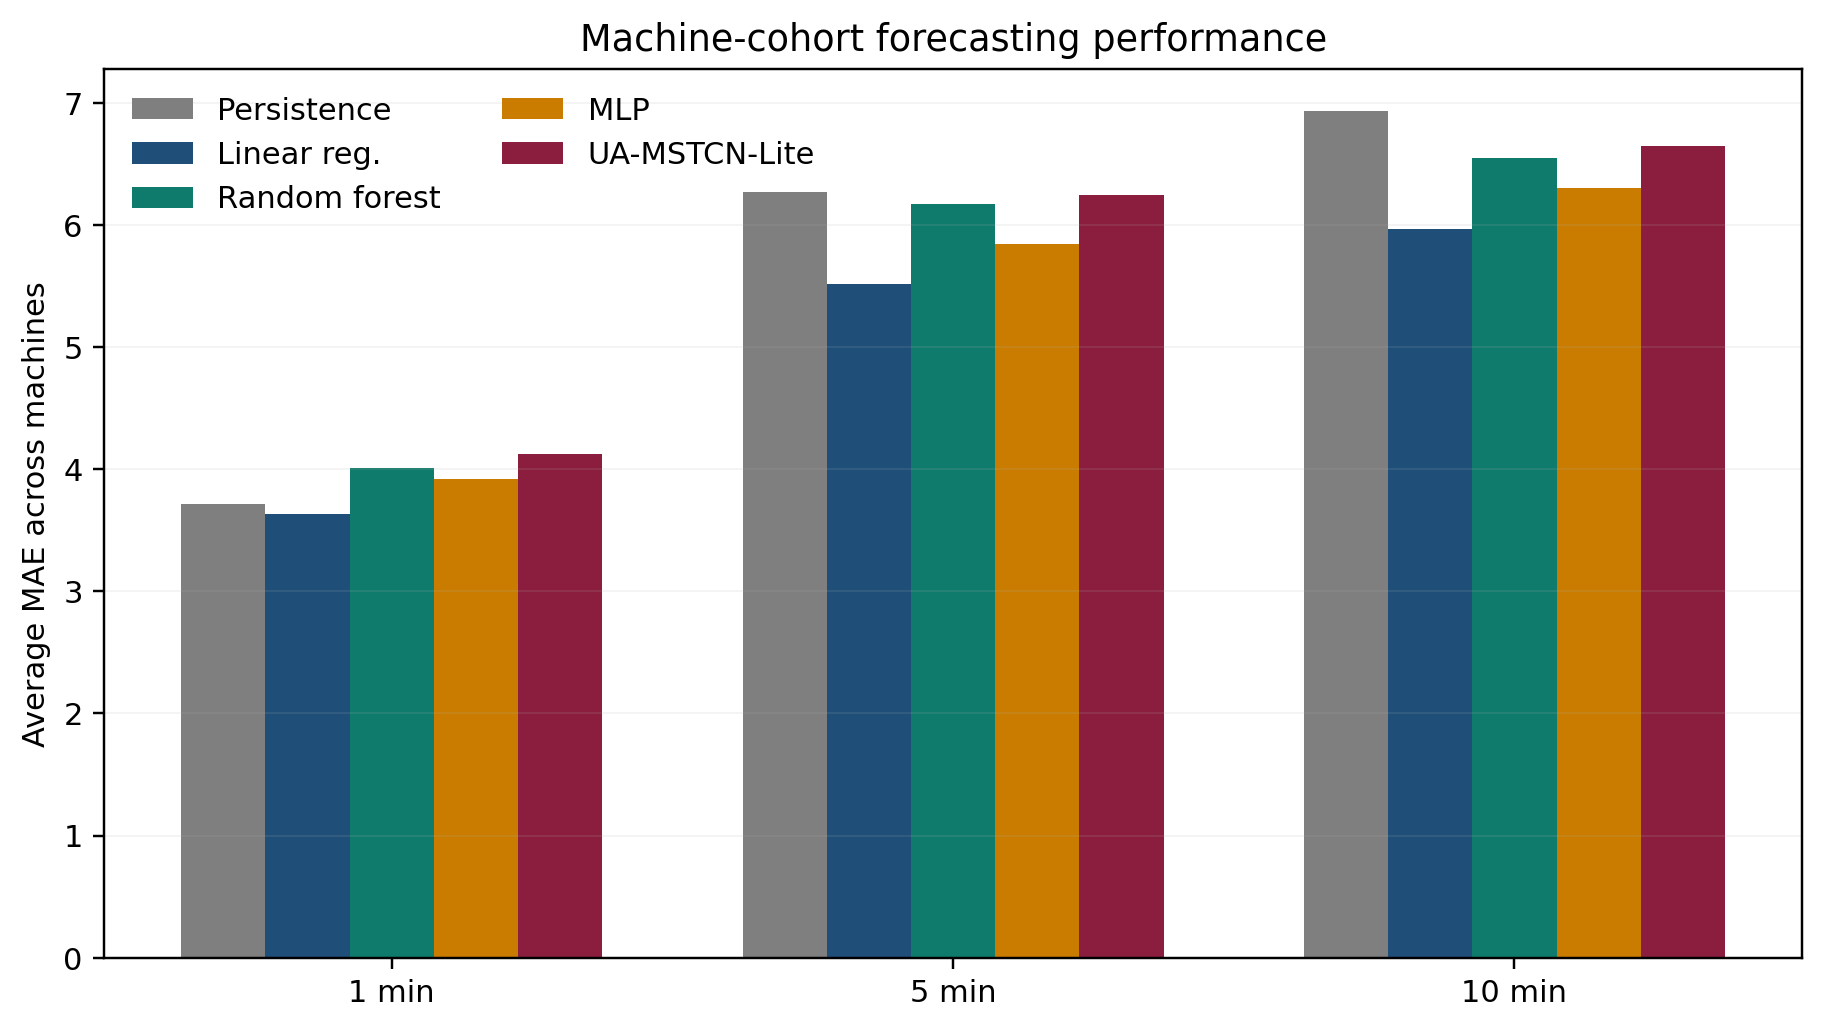
\includegraphics[width=0.78\linewidth]{../experiments/results/machine_cohort/figures/machine_cohort_mae_by_horizon.png}
  \caption{Average forecasting MAE across the 12-machine high-coverage cohort.}
  \label{fig:machine-cohort-mae}
\end{figure}

Figure~\ref{fig:machine-cohort-entity} adds one more view of this heterogeneity. For most machines, \texttt{UA-MSTCN-Lite} remains fairly close to linear regression, but a small subset of entities drives most of the gap. The worst case in the current cohort is \texttt{m\_2014}, where the surrogate's average MAE reaches 9.37 compared with 6.04 for linear regression. This heterogeneity identifies where a deeper temporal model would earn its keep.

\begin{figure}[htbp]
  \centering
  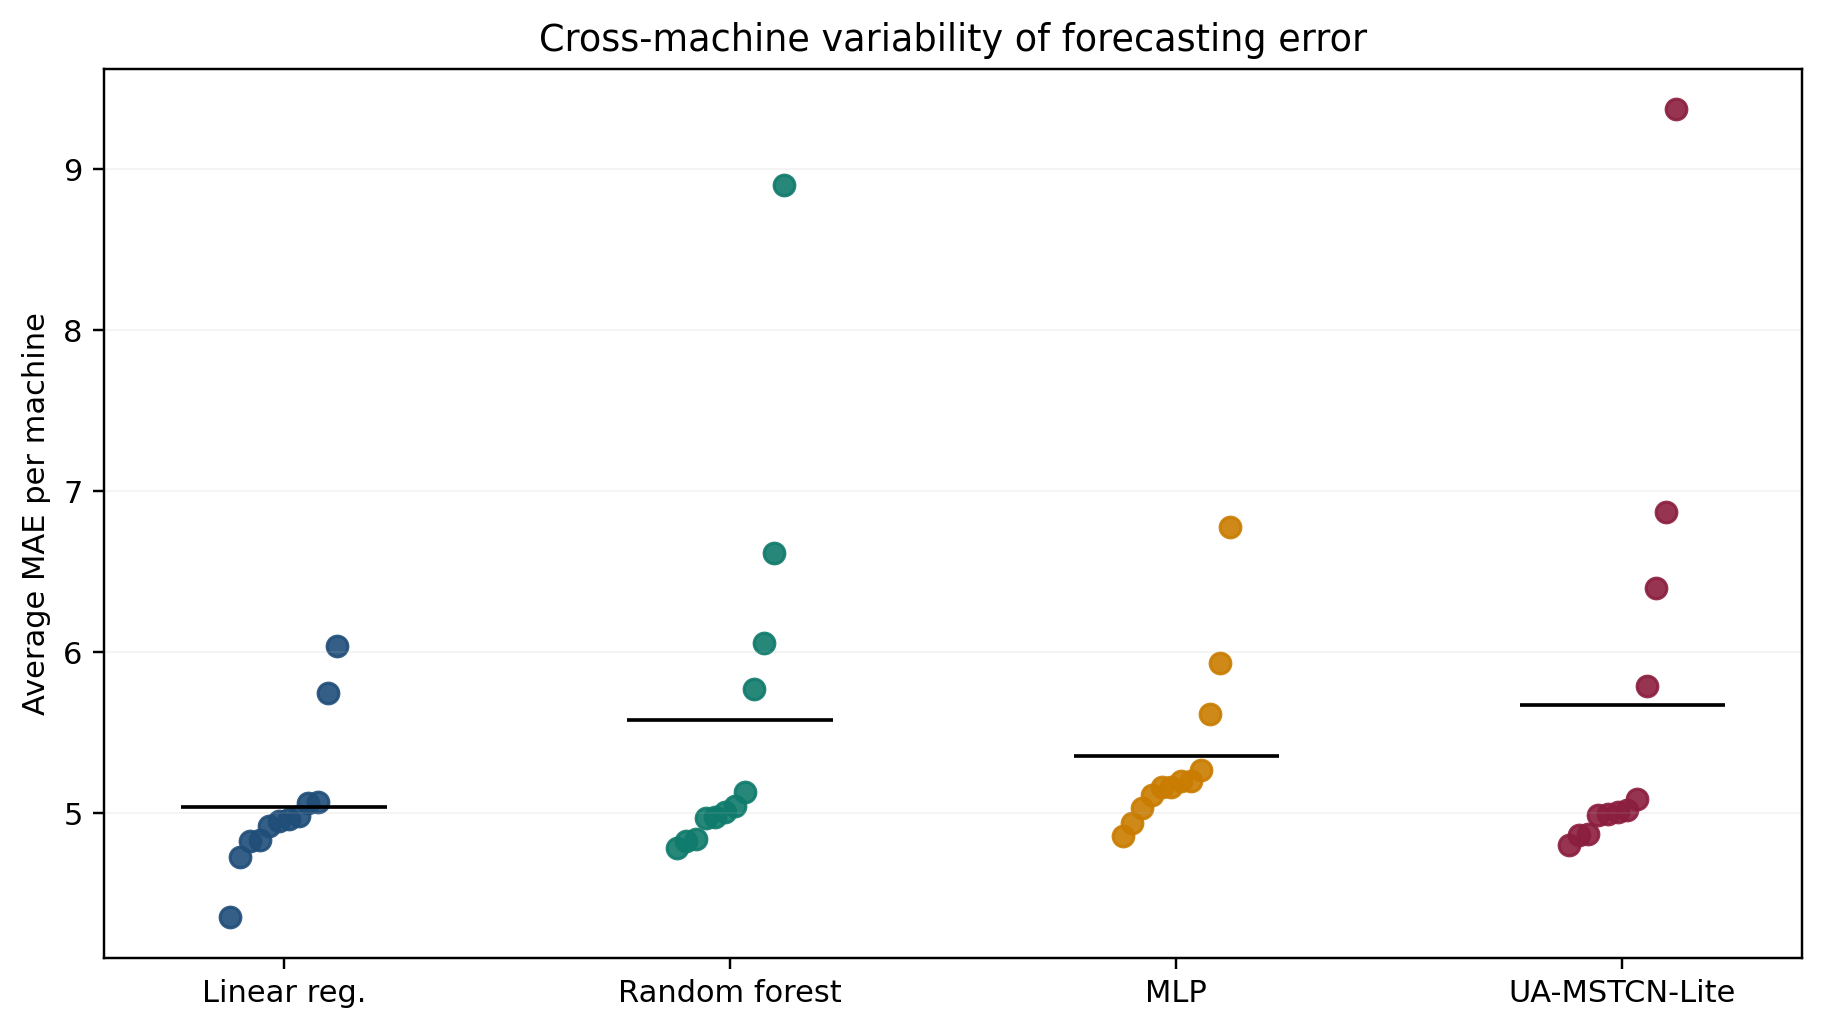
\includegraphics[width=0.78\linewidth]{../experiments/results/machine_cohort/figures/machine_cohort_entity_mae.png}
  \caption{Per-machine average MAE across the 12-machine cohort. Each point is one machine and the horizontal segment marks the model mean.}
  \label{fig:machine-cohort-entity}
\end{figure}

The machine-cohort experiment still supports the uncertainty-aware part of the paper. Table~\ref{tab:machine-cohort-coverage} shows that average $P50$ coverage stays close to 0.5 across horizons and average $P90$ coverage stays between 0.847 and 0.891. The longer-horizon under-coverage is therefore not unique to the aggregate benchmark. This cross-entity pattern strengthens the interpretation that the predictive controller genuinely benefits from an explicit scale-out margin rather than receiving one only as a patch for a single series.

\begin{table}[htbp]
  \centering
  \caption{Average quantile coverage of \texttt{UA-MSTCN-Lite} across the 12-machine cohort.}
  \label{tab:machine-cohort-coverage}
  \scriptsize
  \setlength{\tabcolsep}{3pt}
  \renewcommand{\arraystretch}{0.96}
  \begin{tabular}{lccc}
    \toprule
    Horizon & $P50$ cov. & $P90$ cov. & Mean int. width \\
    \midrule
    1 minute & 0.510 & 0.891 & 7.529 \\
    5 minutes & 0.523 & 0.853 & 9.375 \\
    10 minutes & 0.517 & 0.847 & 9.825 \\
    \bottomrule
  \end{tabular}
\end{table}

\begin{figure}[htbp]
  \centering
  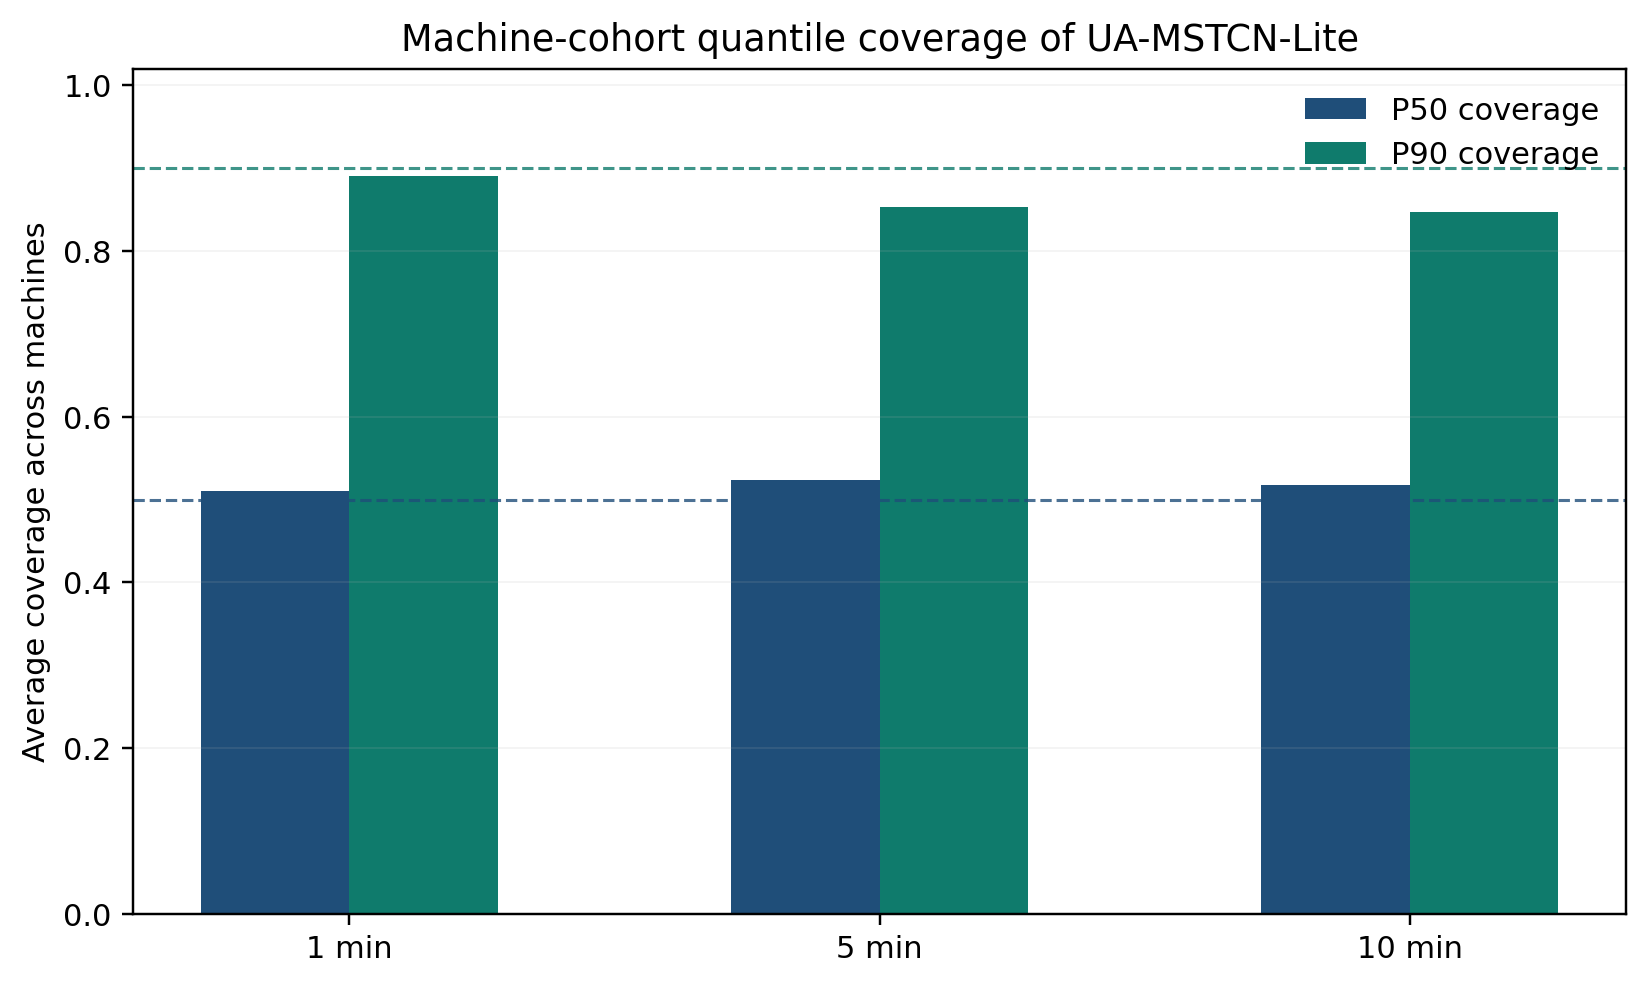
\includegraphics[width=0.72\linewidth]{../experiments/results/machine_cohort/figures/machine_cohort_quantile_coverage.png}
  \caption{Average $P50$ and $P90$ coverage of \texttt{UA-MSTCN-Lite} across the 12-machine cohort.}
  \label{fig:machine-cohort-coverage}
\end{figure}

\subsection{Cross-machine transfer}

The next question is whether forecasting structure learned from one set of machines transfers to unseen machines. To test this, the study runs a 3-fold zero-shot transfer benchmark on the same 12-machine cohort. In each fold, 8 machines are used to train pooled global models and 4 machines are held out entirely for evaluation. Table~\ref{tab:machine-transfer} summarizes the result.

\begin{table}[htbp]
  \centering
  \caption{Cross-machine zero-shot transfer on held-out machines.}
  \label{tab:machine-transfer}
  \tiny
  \setlength{\tabcolsep}{1pt}
  \renewcommand{\arraystretch}{0.96}
  \begin{tabular}{lcccccc}
    \toprule
    Horizon & Pers. & Glob. lin. & Glob. MLP & Glob. RF & Glob. UA & Ent. lin. \\
    \midrule
    1 minute & 3.716 & 3.629 & 3.735 & 4.496 & 3.934 & 3.633 \\
    5 minutes & 6.268 & 5.503 & 5.722 & 6.293 & 6.328 & 5.520 \\
    10 minutes & 6.932 & 5.953 & 6.286 & 6.642 & 6.648 & 5.966 \\
    \bottomrule
  \end{tabular}
\end{table}

The most important observation is not about the uncertainty-aware surrogate. It is that pooled linear regression transfers extremely well across machines. Its mean MAE differs from the entity-specific linear upper bound by only $-0.004$, $-0.017$, and $-0.013$ at the 1-, 5-, and 10-minute horizons, respectively. In other words, the held-out machines in this cohort share enough temporal structure that a simple global linear model generalizes almost perfectly. The global MLP baseline is the next-best zero-shot point predictor, with mean MAE 3.735, 5.722, and 6.286, but it still trails global linear regression at every horizon. This result sets a strong and transparent transfer baseline instead of assuming that a more complex model should dominate by default.

The global \texttt{UA-MSTCN-Lite} model does not beat that baseline on point accuracy, but it still contributes transferable uncertainty estimates. Across held-out machines, its average $P90$ coverage is 0.904, 0.859, and 0.853 for the 1-, 5-, and 10-minute horizons. The same pattern seen in the aggregate and per-machine benchmarks therefore remains visible under zero-shot transfer: point-prediction leadership belongs to the linear baseline, while the uncertainty-aware surrogate remains useful because it exports calibrated quantile bands that a controller can consume.

\begin{figure}[htbp]
  \centering
  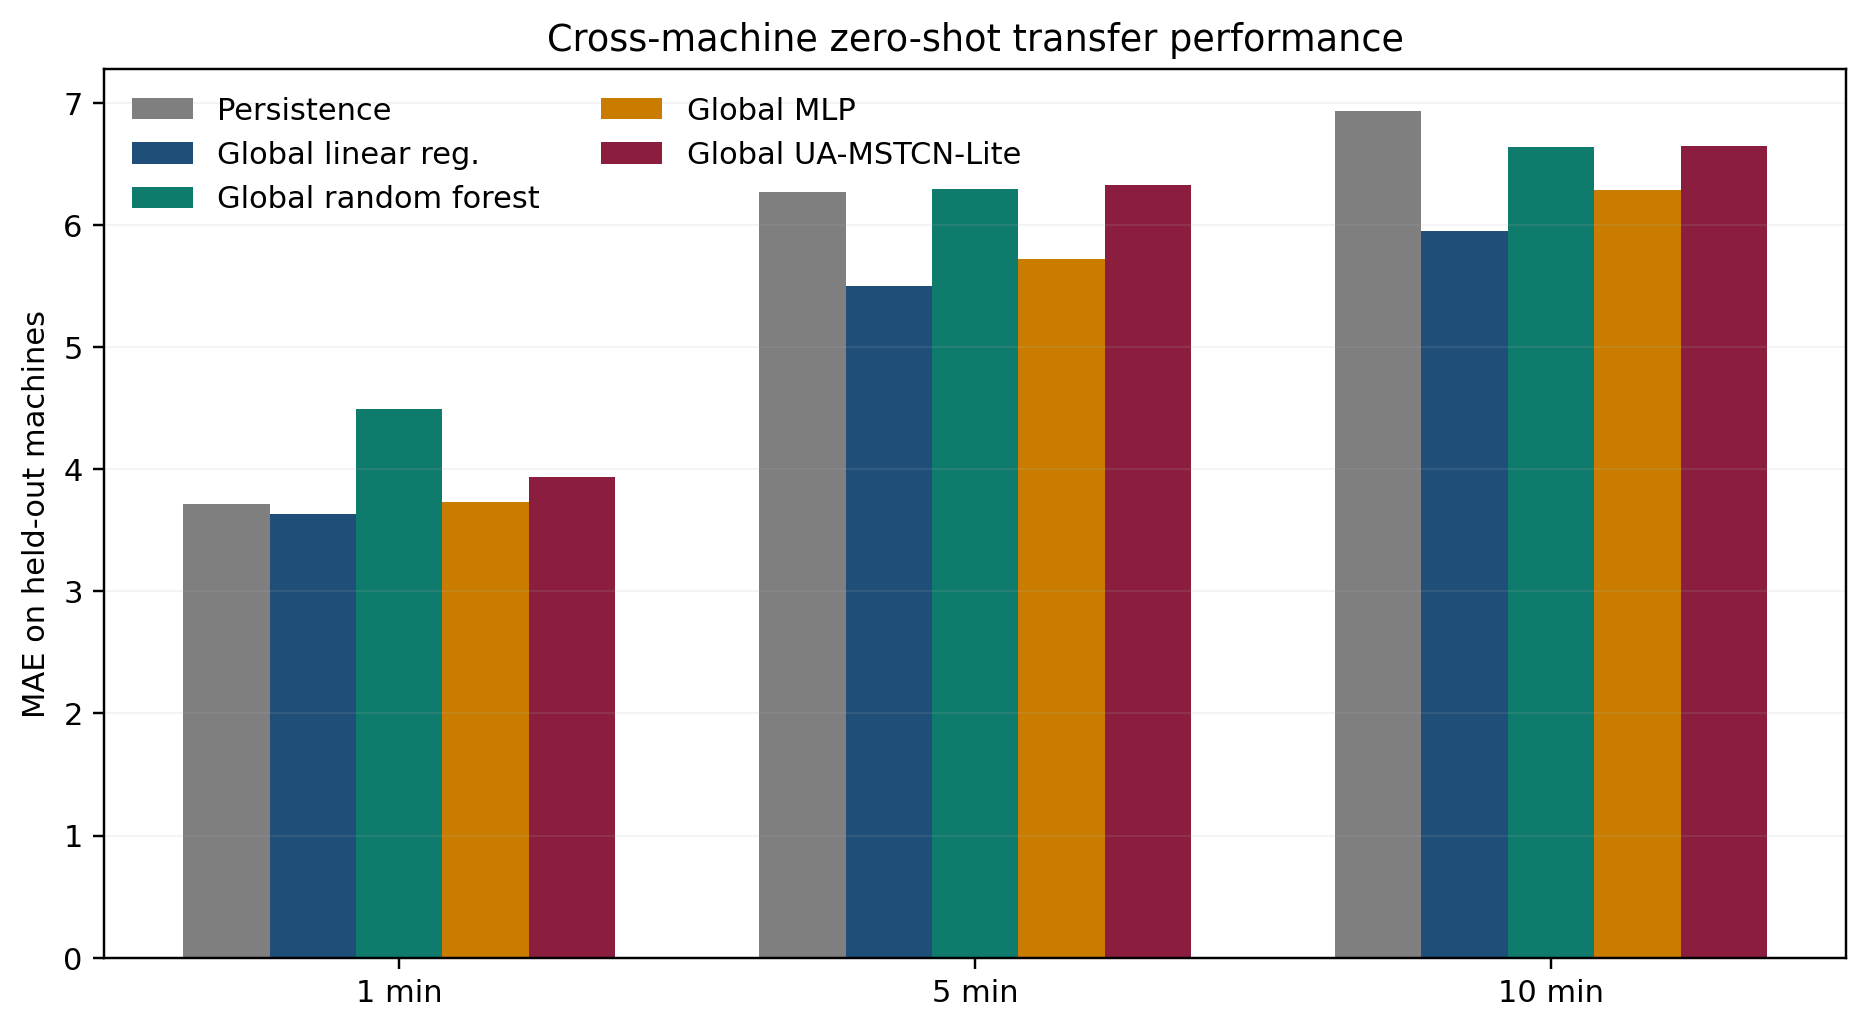
\includegraphics[width=0.78\linewidth]{../experiments/results/machine_transfer/figures/machine_transfer_zero_shot_mae.png}
  \caption{Cross-machine zero-shot transfer performance across the 3 deterministic folds.}
  \label{fig:machine-transfer}
\end{figure}

\subsection{Container service-level evidence}

The construct-validity gap is now materially narrower because the evaluation no longer stops at aggregate and machine abstractions. Using the official \texttt{container\_meta} table together with a full mirrored pass over \texttt{container\_usage}, the study builds a broad service-level cohort covering 139 \texttt{app\_du} groups, 19{,}419 selected containers, 19{,}269 matched containers, and the full shared 11{,}520-minute span introduced in Section~4. A dedicated overlap audit retains all 10 services from the earlier targeted cohort, and the broader audited selection materially changes the service-level conclusions. Table~\ref{tab:service-cohort-promotion} shows that broader service coverage shifts the forecasting winner from \texttt{UA-MSTCN-Lite} to linear regression, turns the scaling-actions delta positive, and leaves the apparent over-provisioning gain unsupported under paired service bootstrap.

\begin{table}[htbp]
  \centering
  \caption{Comparison of service-level conclusions under the earlier targeted top-10 cohort and the broader audited cohort. Deltas are equal-weighted predictive-minus-reactive means.}
  \label{tab:service-cohort-promotion}
  \scriptsize
  \setlength{\tabcolsep}{2pt}
  \renewcommand{\arraystretch}{0.96}
  \begin{tabular}{lcccccc}
    \toprule
    Cohort & Svcs & Cov. & Winner & SLA $\Delta$ & Over $\Delta$ & Acts $\Delta$ \\
    \midrule
    Top-10 & 10 & 0.971 & UA-Lite & +0.033 & -0.720 & -52.4 \\
    Broad & 139 & 0.973 & Linear & +0.014 & -2.633 & +150.4 \\
    \bottomrule
  \end{tabular}
\end{table}

Table~\ref{tab:service-forecasting-summary} summarizes the forecasting result on the audited broad cohort. Linear regression is strongest at every horizon, with MAE 19.999, 34.250, and 43.463 at the 1-, 5-, and 10-minute horizons, respectively. Persistence becomes the overall runner-up at 33.381 average MAE, which is itself a useful warning that local continuity remains a very strong service-level baseline under the broader selection rule. The standard neural MLP baseline does not change that ranking: its average MAE is 37.066, ahead of \texttt{UA-MSTCN-Lite} at 37.787 but behind both linear regression and persistence. The narrower targeted cohort had favored \texttt{UA-MSTCN-Lite}, but that ranking does not survive broader audited service coverage.

\begin{table}[htbp]
  \centering
  \caption{Service-level forecasting across the audited 139-service \texttt{app\_du} cohort.}
  \label{tab:service-forecasting-summary}
  \scriptsize
  \setlength{\tabcolsep}{2pt}
  \renewcommand{\arraystretch}{0.96}
  \begin{tabular}{lcccc}
    \toprule
    Model & 1 min. & 5 min. & 10 min. & Avg. \\
    \midrule
    Persistence & 20.408 & 34.638 & 45.098 & 33.381 \\
    Linear regression & 19.999 & 34.250 & 43.463 & 32.571 \\
    MLP regressor & 23.684 & 38.395 & 49.117 & 37.066 \\
    Random forest & 26.317 & 37.728 & 44.912 & 36.319 \\
    UA-MSTCN-Lite & 27.939 & 39.746 & 45.677 & 37.787 \\
    \bottomrule
  \end{tabular}
\end{table}

Figure~\ref{fig:service-forecasting} shows the same result visually. The more interesting interpretation is not simply that a different model wins. It is that the service traces are much less homogeneous than the aggregate or machine cohorts, and once the selection widens enough, that heterogeneity no longer favors the uncertainty-aware surrogate on point accuracy. This is precisely why a broader service-level extension matters: it reveals that service-level conclusions based on a small targeted subset can move materially once the selection rule is widened and audited.

\begin{figure}[htbp]
  \centering
  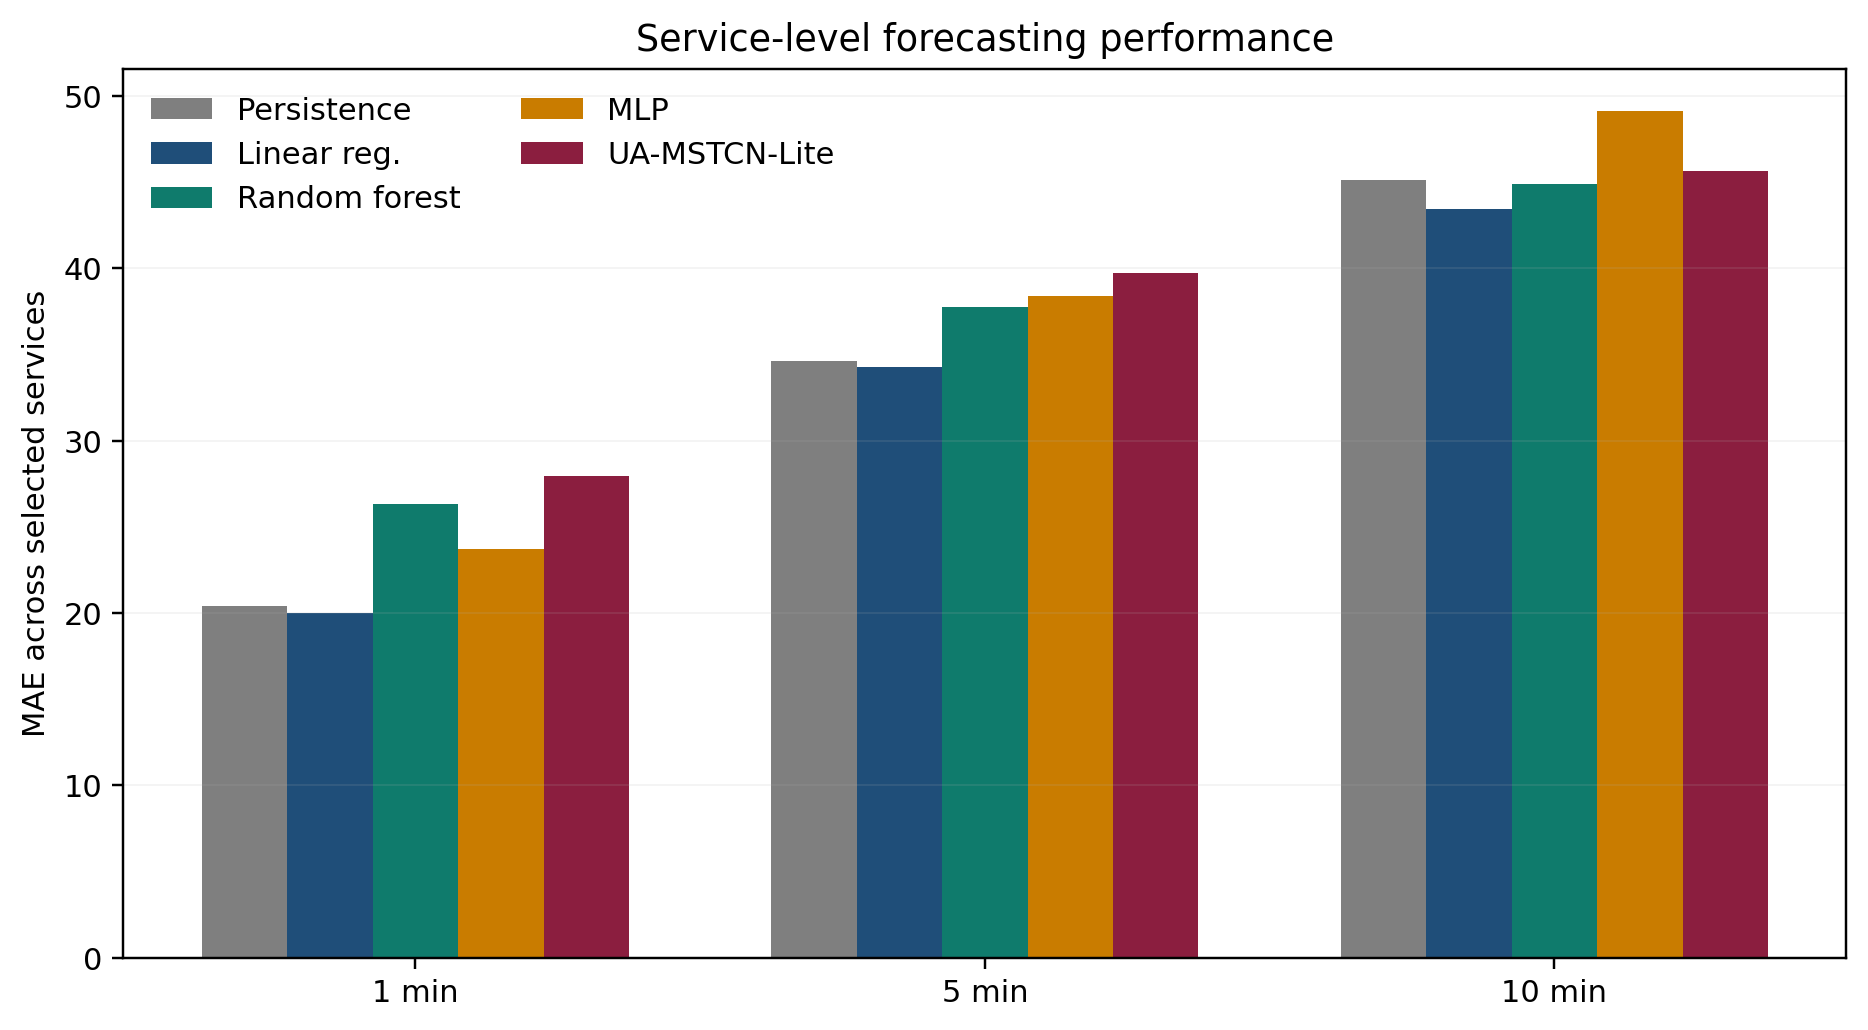
\includegraphics[width=0.82\linewidth]{../experiments/results/service_cohort_broad/figures/service_forecasting_mae.png}
  \caption{Average MAE across the audited 139-service \texttt{app\_du} cohort. Under broader service coverage, point-forecast leadership shifts to linear regression and the generic MLP baseline remains mid-pack rather than dominant.}
  \label{fig:service-forecasting}
\end{figure}

The quantile behavior also remains useful at this finer granularity. Across the 139 services, the empirical $P90$ coverage of \texttt{UA-MSTCN-Lite} is 0.921, 0.896, and 0.877 at the 1-, 5-, and 10-minute horizons, respectively. The median forecasts remain slightly under-centered, with $P50$ coverage between 0.469 and 0.481, but the upper quantile stays close enough to the nominal target to justify its continued use inside the predictive controller even though the model no longer leads on point MAE.

The service-level control comparison is more stringent than the aggregate result because it evaluates the policy under heterogeneous service demand rather than one shared cluster signal. Averaged over the 139 services, the forecast-free lagged target-tracking baseline again marks one extreme of the trade-off surface: it drives over-provisioning down to 3.848 and average reserved capacity down to 124.046, but SLA violation rises to 0.486 and scaling actions explode to 1660.9. Against the operational reactive baseline, the predictive controller raises mean SLA violation from 0.0173 to 0.0311, raises mean scaling actions from 249.0 to 399.4, and raises mean reserved capacity from 164.484 to 178.008, while mean over-provisioning falls from 56.310 to 53.677. The paired service bootstrap makes the conclusion sharper. The equal-weighted predictive-minus-reactive SLA delta is +0.0138 with a 95\% interval of [0.0035, 0.0271], which is a stable degradation. The equal-weighted scaling-actions delta is +150.4 with interval [114.0, 185.0], another stable degradation. The equal-weighted over-provisioning delta remains negative at -2.633, but its interval [-6.953, 2.328] crosses zero, so the apparent over-provisioning gain is not stably supportable under broader service resampling. The auxiliary load-weighted mean scaling-actions delta is nearly zero (-0.567) and also not stable, which suggests that the equal-weighted penalty is driven more by widespread small-service regressions than by the highest-load services alone. At the per-service level, predictive control improves SLA violation for only 27 of 139 services and reduces scaling actions for only 32 of 139, even though it reduces over-provisioning for 95 services. These mixed and negative findings are not incidental; they identify the boundary conditions under which a shared global predictive policy fails under service heterogeneity.

\begin{figure}[htbp]
  \centering
  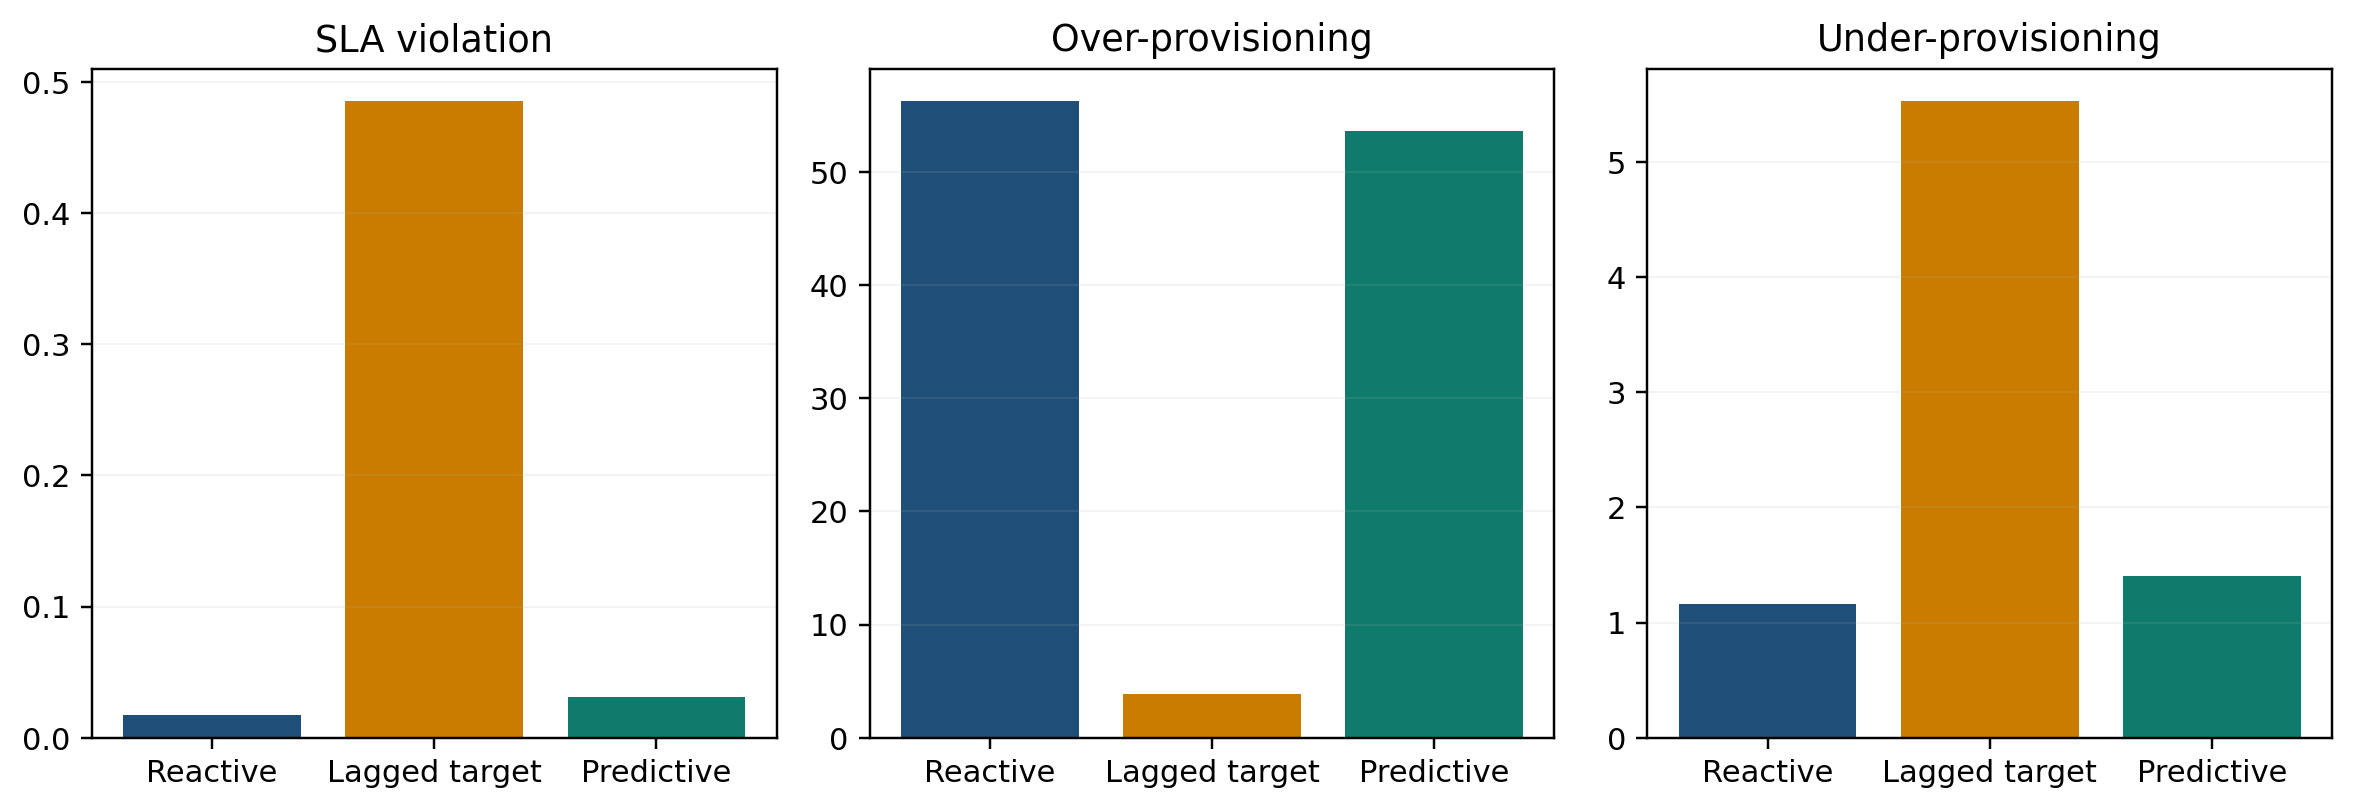
\includegraphics[width=\linewidth]{../experiments/results/service_cohort_broad/figures/service_policy_summary.png}
  \caption{Service-level policy summary across the audited 139-service cohort. The lagged baseline exposes the naive target-chasing extreme, while the predictive controller no longer preserves the earlier service-level action-reduction headline under broader coverage.}
  \label{fig:service-policy-summary}
\end{figure}

\subsection{Trace-driven control comparison}

The aggregate control comparison is driven by a trained uncertainty-aware forecaster rather than by a placeholder forecast source. Table~\ref{tab:policy-results} now summarizes three policies. The reactive threshold policy achieves almost zero SLA violation, but only by carrying a very conservative mean capacity of 0.821 against an average required capacity of 0.470. The lagged target-tracking baseline occupies the opposite extreme: it nearly eliminates over-provisioning (0.013) and keeps mean reserved capacity close to the required load (0.469), but it incurs 47.1\% SLA violation and 1616 scaling actions because one-step-lagged target chasing is too unstable. The predictive policy sits between these extremes. It raises SLA violation to 3.46\%, but cuts over-provisioning by 59.8\% relative to reactive control and keeps mean reserved capacity at 0.610. This is a meaningful systems trade-off rather than an artifact of incomparable units, because all three policies are evaluated in the same normalized required-capacity space and the predictive route applies the same headroom logic to both forecasts and realized demand.

\begin{table}[htbp]
  \centering
  \caption{Reactive, lagged-target, and predictive capacity control on the 5-minute evaluation horizon.}
  \label{tab:policy-results}
  \scriptsize
  \setlength{\tabcolsep}{1.5pt}
  \renewcommand{\arraystretch}{0.96}
  \begin{tabular}{lccccc}
    \toprule
    Policy & SLA & Over & Under & Acts & Cap. \\
    \midrule
    Reactive threshold & 0.001 & 0.351 & 0.000 & 43 & 0.821 \\
    Lagged target tracking & 0.471 & 0.013 & 0.014 & 1616 & 0.469 \\
    Predictive & 0.035 & 0.141 & 0.001 & 589 & 0.610 \\
    \bottomrule
  \end{tabular}
\end{table}

\begin{figure}[htbp]
  \centering
  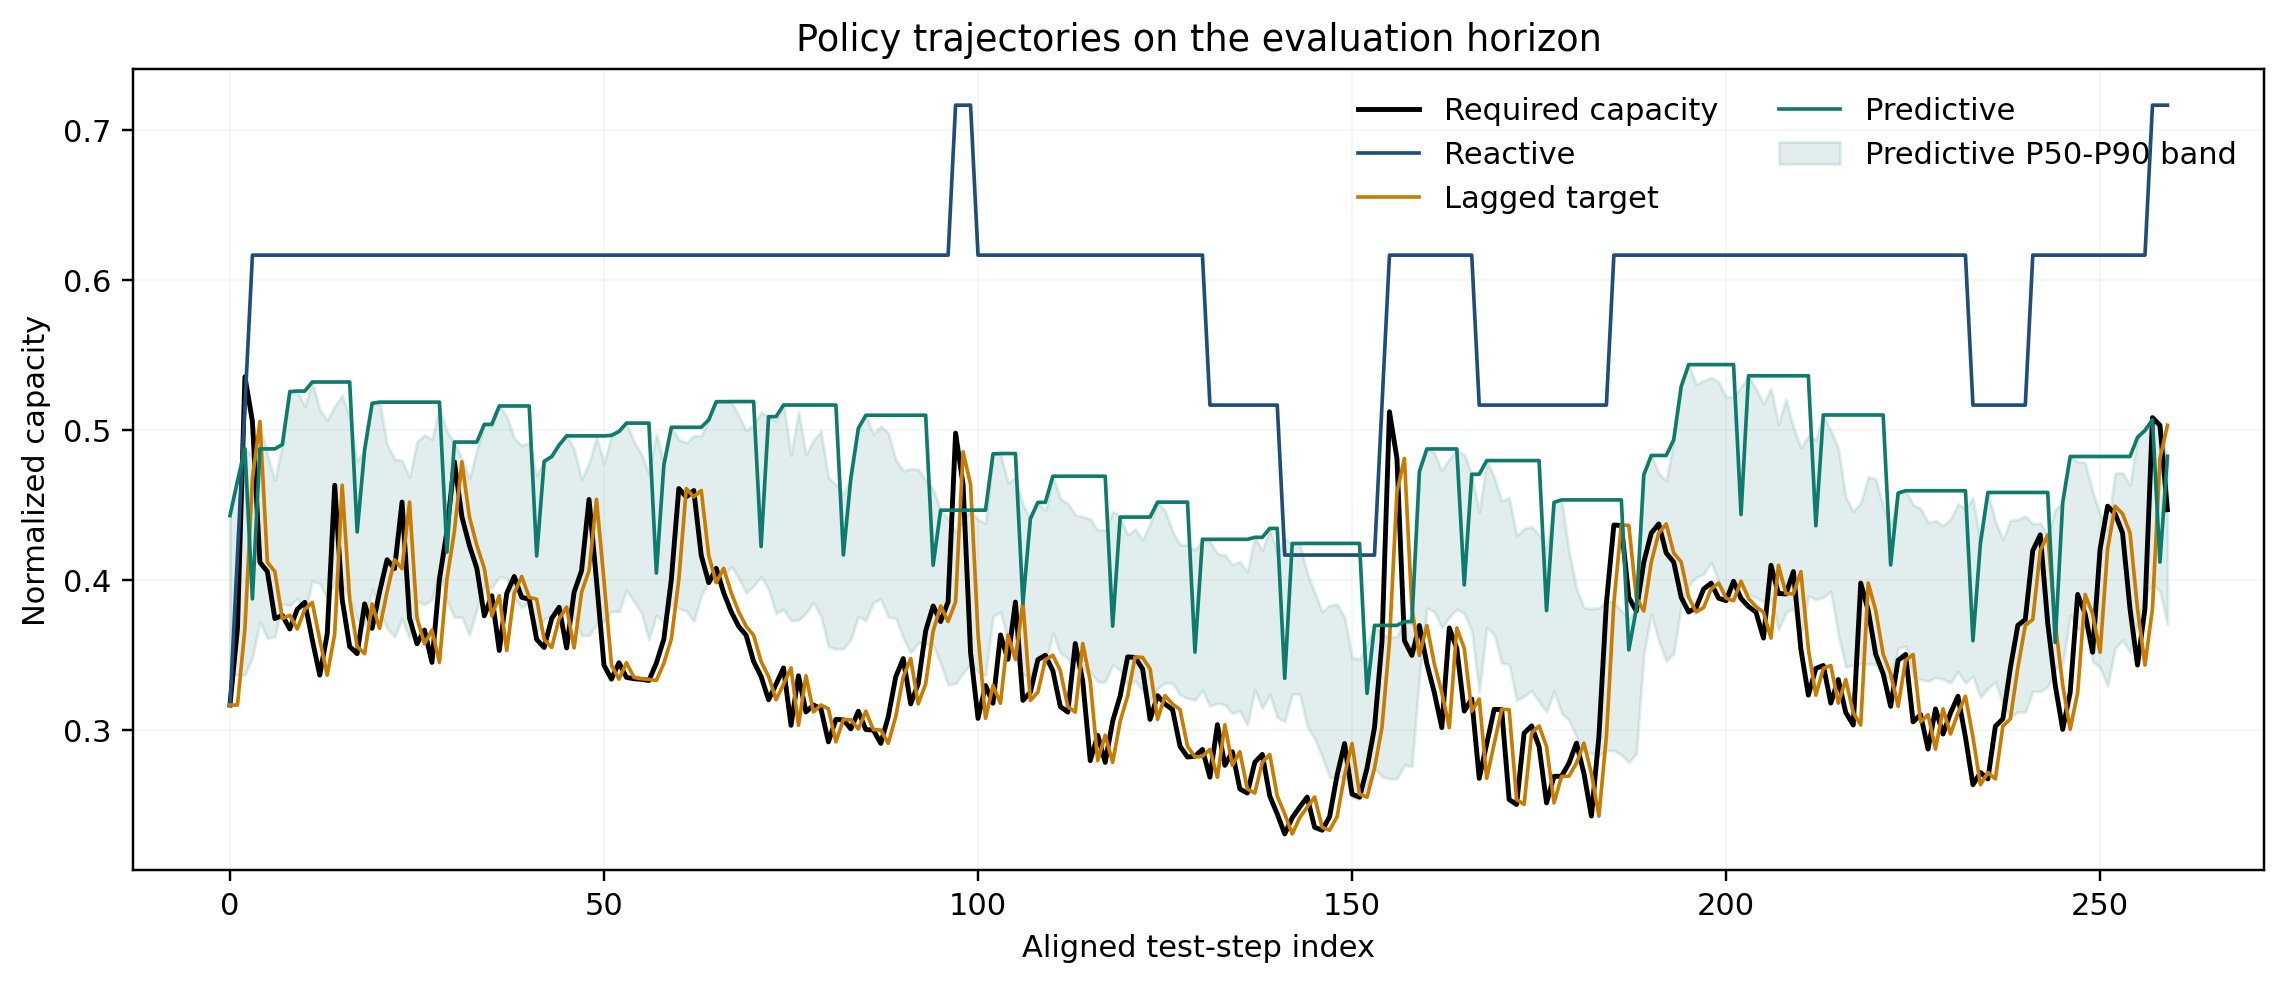
\includegraphics[width=\linewidth]{../experiments/results/figures/policy_capacity_comparison.png}
  \caption{Reactive, lagged-target, and predictive capacity trajectories on the 5-minute evaluation horizon. The lagged baseline shows the failure mode of naive target chasing, while the predictive policy follows the calibrated high-quantile forecast with far lower SLA risk.}
  \label{fig:policy-capacity}
\end{figure}

\subsection{Policy ablation and sensitivity}

The control analysis is now deeper than a single reactive-versus-predictive table. Table~\ref{tab:policy-ablation} shows that the current controller depends heavily on two ingredients: a conservative scale-out margin and cooldown-controlled scale-in. Removing the scale-out margin raises SLA violation from 0.0346 to 0.1137. Removing cooldown keeps over-provisioning relatively low, but pushes the action count from 589 to 1617 and also raises SLA violation to 0.1119. A median-only policy is clearly unacceptable in this setup, with SLA violation rising to 0.3337. By contrast, removing the scale-in guard has almost no effect, which suggests that the current aggregate trace is dominated by scale-out uncertainty rather than scale-in ambiguity.

\begin{table}[htbp]
  \centering
  \caption{Predictive-policy ablation on the 5-minute evaluation route.}
  \label{tab:policy-ablation}
  \scriptsize
  \setlength{\tabcolsep}{1.5pt}
  \begin{tabular}{p{1.65cm}ccccc}
    \toprule
    Variant & SLA & Over & Under & Acts & Cap. \\
    \midrule
    Full predictive policy & 0.035 & 0.141 & 0.001 & 589 & 0.610 \\
    No scale-out margin & 0.114 & 0.089 & 0.004 & 589 & 0.555 \\
    No cooldown & 0.112 & 0.100 & 0.005 & 1617 & 0.565 \\
    Median only & 0.334 & 0.035 & 0.017 & 359 & 0.488 \\
    No scale-in guard & 0.035 & 0.141 & 0.001 & 589 & 0.610 \\
    \bottomrule
  \end{tabular}
\end{table}

Figure~\ref{fig:policy-pareto} extends the same argument with a sweep over scale-out margin and cooldown settings. The chosen default point $(m=0.10, c=8)$ is not globally optimal on any single axis, but it sits near the middle of the observed Pareto surface. Smaller margins reduce over-provisioning but push SLA risk sharply upward, while larger margins and longer cooldown improve SLA protection by consuming more steady capacity. This is exactly the kind of operational trade-off that a systems paper should make explicit rather than hide behind a single best configuration.

\begin{figure}[htbp]
  \centering
  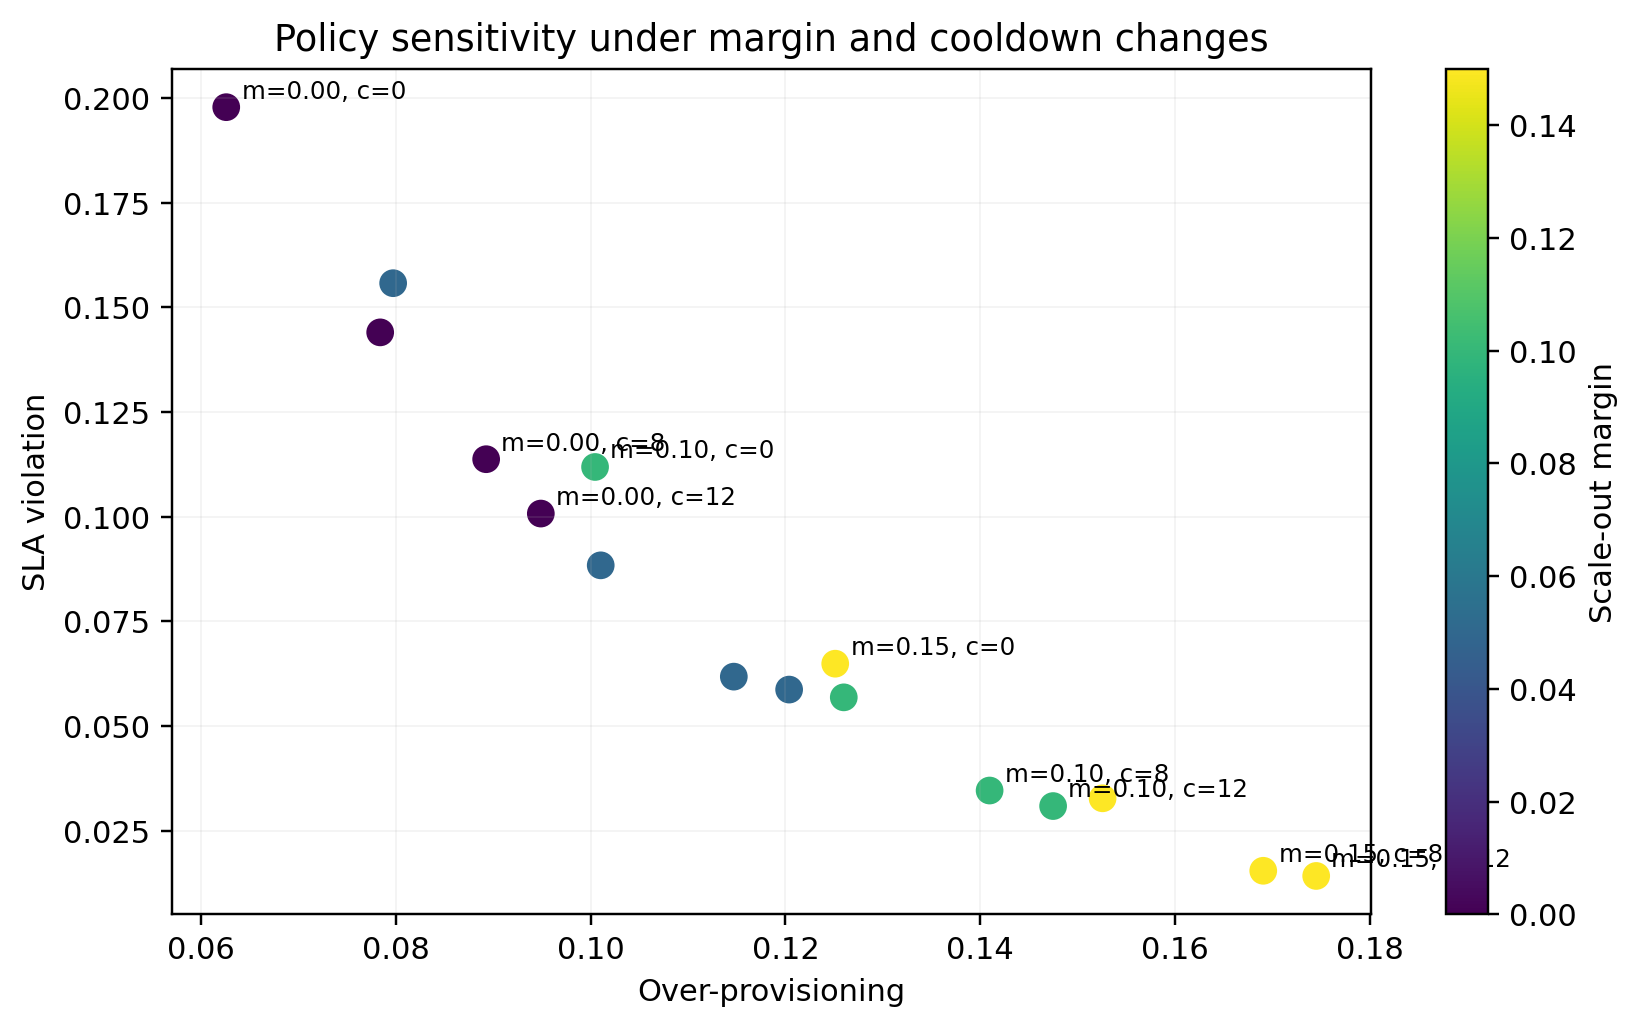
\includegraphics[width=0.82\linewidth]{../experiments/results/figures/policy_pareto_sensitivity.png}
  \caption{Sensitivity of the predictive controller to scale-out margin and cooldown. The selected default operates in the middle of the observed SLA-versus-over-provisioning trade-off.}
  \label{fig:policy-pareto}
\end{figure}

The boundary is now narrower. A public trace-driven simulator with a trained forecasting backbone, calibration evidence, and policy ablations is strong evidence for reproducible control trends, but it is still not a substitute for a live production deployment. The current result should therefore be interpreted as trace-level evidence about when predictive control succeeds and when it fails, not as proof that the same policy would transfer unchanged to a real cluster controller.


\section{Threats to Validity}
Several validity threats remain.

\paragraph{External validity.}
The study uses public Alibaba traces rather than a live platform, so the conclusions are strongest for trace-driven comparison and weaker for direct deployment claims.

\paragraph{Construct validity.}
The service cohort narrows the construct-validity gap but is not a full service census. It is bounded by a metadata prefilter requiring at least 60 containers and 650{,}000 seconds of span, followed by usage-profile and post-aggregation quality thresholds. The benchmark should therefore be read as a broad rule-based service cohort, not the full \texttt{app\_du} population.

\paragraph{Internal validity.}
\texttt{UA-MSTCN-Lite} is a lightweight trainable surrogate, not the final deep UA-MSTCN architecture. The reported numbers therefore apply to the verified surrogate and policy route, not to an unimplemented deeper model.

\paragraph{Conclusion validity.}
Forecasting gains do not automatically imply better capacity control, so forecasting and policy metrics are kept separate. The service-descriptor splits and taxonomy are descriptive benchmark analyses, not causal identification for live services.


\section{Conclusion}
This paper contributes a reproducible public-trace benchmark for predictive autoscaling across aggregate, machine-level, transfer, and broad service-level evidence. Linear regression remains the strongest point-forecast baseline across the main benchmarks, while \texttt{UA-MSTCN-Lite} contributes calibrated upper quantiles for predictive control.

The central contribution is therefore boundary mapping rather than a new controller architecture. Aggregate predictive control reduces over-provisioning relative to reactive control, but the audited 139-service cohort shows higher mean SLA violation and scaling actions, with no stable over-provisioning gain under paired service bootstrap. Descriptor splits locate the harshest SLA penalties in burstier and more persistent services and the clearest over-provisioning relief in lower-load and lower-burstiness halves.

Next steps are service-aware tuning under held-out-service evaluation and a stronger temporal backbone tested against the same linear and persistence baselines.


\section*{Statements and Declarations}
\paragraph{Funding}
The author received no specific funding for this study.

\paragraph{Competing interests}
The author declares no competing interests.

\paragraph{Ethics approval and consent to participate}
Not applicable.

\paragraph{Consent for publication}
Not applicable.

\paragraph{Data availability}
The raw Alibaba Cluster Trace Program datasets are publicly available from the Alibaba Cluster Trace Program repository. The submitted manuscript version is maintained in a private GitHub review repository together with a frozen review-freeze package that includes processed datasets, cohort summaries, result tables, figure-generation artifacts, and manuscript sources. Access can be granted to the editor and reviewers during peer review. Upon acceptance, the same frozen package will be deposited in a public repository with a persistent identifier.

\paragraph{Materials availability}
Not applicable.

\paragraph{Code availability}
The scripts used for preprocessing, forecasting, broad service-cohort construction, and policy evaluation are maintained in the same private GitHub review repository and frozen review-freeze package. Access can be granted to the editor and reviewers during peer review. Upon acceptance, the same code package will be deposited in the same public repository with a persistent identifier.

\paragraph{Author contribution}
Jinchun Liu conceived the study, designed the methodology, implemented the experiments, analyzed the results, and wrote the manuscript.


\bibliography{refs}

\end{document}
